%!TEX TS-program = xelatex
\documentclass[a4paper,12pt]{article}
\usepackage[left=30mm, top=30mm, right=30mm, bottom=30mm, nohead, nofoot]{geometry}
\usepackage[OT6, T1]{fontenc}
\usepackage[utf-8]{inputenc}
\usepackage[english,russian]{babel}%% загружает пакет многоязыковой вёрстки
\newcommand{\armenian}{\fontencoding{OT6}\fontfamily{cmr}\selectfont}
\DeclareTextFontCommand{\textarmenian}{\armenian}


\usepackage{fontspec}
\setmainfont[
BoldFont=brillb.ttf,
ItalicFont=brilli.ttf,
BoldItalicFont=brillbi.ttf
]{brill.ttf}
	
	%%% Дополнительная работа с математикой
    \usepackage{float}
	\usepackage{amsmath,amsfonts,amssymb,amsthm,mathtools} % AMS
	\usepackage{icomma} % "Умная" запятая: $0,2$ --- число, $0, 2$ --- перечисление
	
	%%% Работа с картинками
	\usepackage{wrapfig} % Обтекание рисунков текстом
	\usepackage{subcaption}
	\usepackage{rotating}
	\usepackage{hhline}
	\usepackage{lscape}
	\usepackage[usenames,dvipsnames,svgnames,table,rgb]{xcolor}%пакет для использования цветов

	\usepackage[inline]{enumitem}
	
	%%% Работа с таблицами
	\usepackage{array,tabularx,tabulary,booktabs} % Дополнительная работа с таблицами
	\usepackage{longtable} % Длинные таблицы
	\usepackage{multirow} % Слияние строк в таблице
	
	\usepackage{multicol} % Несколько колонок
	
	%%% Страница
	\usepackage{extsizes} % Возможность сделать 14-й шрифт
	\usepackage{geometry} % Простой способ задавать поля
	\geometry{top=20mm}
	\geometry{bottom=20mm}
	\geometry{left=20mm}
	\geometry{right=20mm}
	
	%\usepackage{fancyhdr} % Колонтитулы
	% \pagestyle{fancy}
	%\renewcommand{\headrulewidth}{0pt} % Толщина линейки, отчеркивающей верхний колонтитул
	% \lfoot{Нижний левый}
	% \rfoot{Нижний правый}
	% \rhead{Верхний правый}
	% \chead{Верхний в центре}
	% \lhead{Верхний левый}
	% \cfoot{Нижний в центре} % По умолчанию здесь номер страницы
	
	\usepackage{setspace} % Интерлиньяж
	\onehalfspacing % Интерлиньяж 1.5
	%\doublespacing % Интерлиньяж 2
	%\singlespacing % Интерлиньяж 1
	
	\usepackage{lastpage} % Узнать, сколько всего страниц в документе.
	\usepackage{soul} % Модификаторы начертания
	\usepackage{bbding}
	\definecolor{dark-gray}{gray}{0.3}
	\usepackage{hyperref}
	\usepackage[usenames,dvipsnames,svgnames,table,rgb]{xcolor}
	\hypersetup{ % Гиперссылки
	colorlinks=true, % false: ссылки в рамках; true: цветные ссылки
	linkcolor=dark-gray, % внутренние ссылки
	citecolor=black, % на библиографию
	filecolor=black, % на файлы
	urlcolor=ForestGreen % на URL
	}
	
	\usepackage{environ}
	\makeatletter
	\newsavebox{\measure@tikzpicture}
	\NewEnviron{scaletikzpicturetowidth}[1]{%
	\def\tikz@width{#1}%
	\def\tikzscale{1}\begin{lrbox}{\measure@tikzpicture}%
	\BODY
	\end{lrbox}%
	\pgfmathparse{#1/\wd\measure@tikzpicture}%
	\edef\tikzscale{\pgfmathresult}%
	\BODY
	}
	\makeatother
	
    \usepackage{verbatim}
	
	\usepackage{attachfile2}
	\attachfilesetup{appearance=true,
	color=0 0 0
	}
	
	%%% Лингвистические пакеты
	%\usepackage{savetrees} % пакет, который экономит место
	\usepackage{forest} % для рисования деревьев
	\usepackage{vowel} % для рисования трапеций гласных
	\usepackage{natbib}
	\bibpunct[: ]{[}{]}{;}{a}{}{,}

	\usepackage{philex} % пакет для примеров
    
	\renewcommand{\thesection}{\arabic{section}.}
	\renewcommand{\thesubsection}{\arabic{section}.\arabic{subsection}}
	\setlength{\columnsep}{1.6cm}
	
	\usepackage{sectsty}
	\sectionfont{\normalsize}
	\subsectionfont{\normalsize}
	\usepackage{titlesec}
	\titlespacing*{\section}
	{0pt}{2ex plus 0ex minus .2ex}{0ex plus .2ex}
	\titlespacing*{\subsection}
	{0pt}{2ex plus 0ex minus .2ex}{0ex plus .2ex}
	\newlength{\bibitemsep}\setlength{\bibitemsep}{.2\baselineskip plus .05\baselineskip minus .05\baselineskip}
	\newlength{\bibparskip}\setlength{\bibparskip}{0pt}
	\let\oldthebibliography\thebibliography
	\renewcommand\thebibliography[1]{%
	\oldthebibliography{#1}%
	\setlength{\parskip}{\bibitemsep}%
	\setlength{\itemsep}{\bibparskip}%
	}
\usepackage{tikz}
\usetikzlibrary{arrows,positioning,shapes.geometric}
\usepackage{longtable}


\usepackage{alltt}
\usepackage{bibunits}
\usepackage{enumitem}
\usepackage{ltablex,booktabs}
\begin{document}
\definecolor{zzttqq}{rgb}{0.26666666666666666,0.26666666666666666,0.26666666666666666}
\definecolor{cqcqcq}{rgb}{0.7529411764705882,0.7529411764705882,0.7529411764705882}
\thispagestyle{empty}
\begin{center}
\noindent 
\textbf{Правительство Российской Федерации \\Федеральное государственное автономное образовательное учреждение высшего образования}

\textbf{Национальный исследовательский университет}\\
\textbf{«Высшая школа экономики»}\\
\textbf{Факультет гуманитарных наук}\bigskip\\
\vfill
Образовательная программа \\
  «Фундаментальная и компьютерная лингвистика»\\
\vfill

\huge{КУРСОВАЯ РАБОТА}\\
\large

На тему \\
\Large
«Туман и его разновидности: типология лексикализации одного природного явления»\\
«Fog and its variations: the typology of the natural phenomenon's lexicalization»\\
\vfill
\vfill
\normalsize
\begin{flushright}
Студент 3 курса\\
группы №153 \\
Соколовский Матвей Ильич\bigskip\\
                       
Научный руководитель\\
канд. филологических наук, доц.\\
Резникова Татьяна Исидоровна\\

\end{flushright}
\vfill
\begin{center}
Москва --- 2018
\end{center}

\end{center}
\pagebreak
{
  \hypersetup{linkcolor=black}
  \tableofcontents
}
\pagebreak

\section{Введение} 
\subsection{Общее} \label{preview}

\par В основу данной работы легла курсовая работа прошлого года в которой представлены первые попытки исследования семантического поля 'облака, тучи туман' \citep{соколовский2017}. Метод семантического картирования, использовавшийся как в прошлой, так и в нынешней работе, описан в статье С.Г. Татевосова \citep{татевосов2004}, однако рассматривался и ранее, к примеру, в масштабной книге о лингвистической типологии Мартина Хаспельмата \citep{haspelmath2001language}. В статье Йохана Ауверы и Владимира Плунгяна о типологии модальности \citep{van1998modality} можно увидеть применение метода семантического картирования в грамматической типологии. Подробнее о применении метода к лексическому материалу: \citep{рр2013}. Также, в статьях \citep{krv2015}, \citep{плунгян2007} представлен более широкий обзор направления лексической типологии и применимых к нему методов.

\par Многое в лексической типологии, несмотря на её сравнительную молодость, уже сделано. Однако чаще внимание лексических типологов привлекают глагольные семантические поля (ср. \citep{майсак2007глаголы}, \citep{кузьменко2015глаголы}, \citep{багдасарянглаголы}, а также классические работы \citep{newman2009linguistics} и \citep{majid2007semantic}), либо семантические поля прилагательных (\citep{архангельский2011качественные}, \citep{кюсева2010признаковая}). На сайте \hyperlink{mlext}{проекта MLexT} можно также найти ряд работ, посвящённых по большей части признаковым семантическим полям. В исследованиях семантических полей глаголов и прилагательных значительно лучше применимы методы дистрибутивной семантики, основанные на контекстной сочетаемости лексем. В первую очередь это связано с тем, что достаточно просто посмотреть существительные, способные выступать в качестве спецификатора рассматриваемого нами глагола, или существительные, способные присоединять к себе рассматриваемое нами прилагательное. Однако не так очевидно, какого рода сочетаемость позволит выделить фреймы для существительных. Модели дистрибутивной семантики позволяют делать существенные шаги в направлении автоматизации подобного рода исследований (см. \citep{орехов2015компьютерные} и \citep{рыжова2018автоматизация}), но исследование именного семантического поля до сих пор требует большого количества ручной работы. 
\par В качестве примера работ, рассматривавших ранее именные семантические поля можно привести ранние \citep{greenberg1990universals} и \citep{koch1999tree}. А также более современное исследование лексикализаций оболочек предметов \citep{шкурныйвопрос}, в котором также применён метод фреймового подхода. Однако типология лексикализаций природных явлений ни в одной работе ранее не рассматривалась.

\par Основным результатом работы \citep{соколовский2017} можно считать набор релевантных фреймов и семантическую карту для семантического поля 'облака, тучи, туман'. Наиболее неожиданные данные были получены в зоне, которая соответствует русской лексеме туман: для этой подзоны было выделено 5 фреймов. На основании данных о группе европейский языков (голландский, английский, французский) была проведена граница между туманом, окружающим наблюдателя, и туманом, находящимся в отдалении. В испанском языке обнаружилось деление туманов "по температуре", то есть лексема, применимая исключительно к туману \textit{(дымке)} возникающему на море в тёплую погоду. Возникновение пятого фрейма обусловлено данными армянского языка, в котором наблюдалось противопоставление \textit{туманов окружающих наблюдателя} по густоте (ср. \textit{марево})

\par Однако, в рамках предыдущего исследования, охватывавшего широкое концептуальное пространство, у нас не было возможности в деталях изучить эту частную семантическую область, поэтому, к примеру, не рассматривались лексемы, относящиеся к периферии этой зоны (ср. в русском \textit{марево, дымка}). Также можно сказать, что распределение языкового материала по фреймам было в некоторой степени условным (в первую очередь касательно армянского языка). Противопоставление некоторых фреймов (в частности выделение двух типов "тёплого" тумана) не кажется достаточно точным. Таким образом, анализ семантического поля "туман" требует существенной доработки. 

\par Богатство лексикализаций в армянском языке навело на гипотезу, которую можно сформулировать следующим образом: "семантическое поле \textit{туман} богаче в языках, развивавшихся и распространённых на территории с более горной местностью". Идея представляется логичной по той причине, что из всех языков, рассматривавшихся в \citep{соколовский2017}, только армянский развивался и распространён поныне на преимущественно горной местности. 

\par Таким образом, данная работа ставит перед собой сразу ряд целей:
\begin{enumerate}
\item Уточнить данные армянского языка, в частности, распределение лексем по фреймам.
\item Собрать и рассмотреть данные о новых языках, которые можно условно отнести к \textit{горным}, иными словами, развивавшимся и сохранившимся на территории с преимущественно горной местностью. Тем самым планируется проверить гипотезу, сформулированную выше.
\item Расширить описание семантического поля "туман" для некоторых рассматривавшихся ранее языков, исследовав с помощью корпусов и словарей употребление лексем, обозначающих разновидности лёгкого тумана. (англ. \textit{haze, mist}; рус. \textit{дымка, марево, смог} и проч.) 
\item На примере нескольких языков изучить богатство метафорических значений лексем, относящихся к рассматриваемому полю.
\end{enumerate}

\subsection{Методы работы} \label{methods}
\par Метод, построенный преимущественно на анкетировании носителей, применялся в предыдущей работе и давал неплохие результаты. В области лексической типологии, как отмечалось в \citep{рыжова2015построение}, анкетирование можно считать наиболее эффективным методом сбора данных. Таким образом, было решено применить его повторно, с учётом тех сложностей, которые возникали в ходе предыдущей работы.

\par Первоочередная проблема, возникающая в ходе подобного сбора данных – большое количество не относящегося к теме материала, как например для рис. \hyperlink{p10}{10} использованного как в предыдущей, так и в нынешней анкете, многие давали ответы обозначающие ясную погоду, синее небо, тогда как ожидалось название облака. Для её решения была составлена более подробная инструкция по заполнению анкеты, а также добавлена возможность прокомментировать любое своё словоупотребление. Набор изображений-стимулов увеличился с 9 (в \citep{соколовский2017}) до 16 (с рис. \ref{fig:r1} по рис. \ref{fig:r16} в разделе \ref{приложение}). В новом опросе изображения-стимулы с туманами выдавались поочерёдно и в случайном порядке. Таким образом было снижено влияние порядка изображений опроса на финальный результат. Подробнее о \hyperlink{form}{сайте с опросом} можно узнать на \hyperlink{github}{странице проекта на Github}.


\par С помощью опроса были собраны данные по русскому, финскому, грузинскому, армянскому и каратинскому \footnote{Язык каратинцев. Относится к нахсхо-дагестанской семье и насчитывает всего около 250 носителй.} языкам, и они рассматриваются в разделе \ref{армянский}. В разделе \ref{корпус} с применением всех доступных корпусных методов мы рассматриваем богатство лексем и метафор в русском, английском и немецком языках. Русские лексемы анализировались в русском веб-корпусе ruTenTen$11$ на базе \hyperlink{tenten}{Sketch Engine}, сервисе вычисляющем семантическую близость на основе дистрибутивных методов  \hyperlink{rusvectores}{RusVectōrēs} \citep{KutuzovKuzmenko2017} и основном корпусе \hyperlink{ruscorpora}{НКРЯ}. Об английском и немецком данные по большей части взяты из параллельных корпусов \hyperlink{ruscorpora}{НКРЯ} а также из корпусов deTenTen$13$ и BNC на базе \hyperlink{tenten}{Sketch Engine}. Раздел \ref{semap} представляет из себя попытку соединения всех рассмотренных данных в виде составления набора фреймов и нанесения данных на семантические карты.

\section{Картина в корпусных языках} \label{корпус}

\subsection{Русские лексемы "лёгких" туманов} \label{rus}

\par Итак, как уже было сказано, в работе \citep{соколовский2017} рассматривалась только русская лексема \textit{туман}, так что первым делом рассмотрим семантически близкие к ней существительные русского языка. К ним можно отнести слова \textit{дымка}, \textit{марево}, \textit{мгла}, а также заимствованное \textit{смог}. Количество вхождений в \hyperlink{tenten}{ruTenTen} составляет: 293 тысячи для лексемы \textit{туман}, примерно по 44 тысячи для лексем \textit{дымка} и \textit{мгла} и около 12 тысяч для лексем \textit{марево} и \textit{смог}. На основании одних этих цифр можно сделать вывод о том, что \textit{туман} является базовым словом для всего поля. Для сравнения, лексема \textit{дым}, содержащаяся в условном списке "базовой" лексики, списке Сводеша, насчитывает в \hyperlink{tenten}{ruTenTen} 387 тысяч вхождений. В связи с этим мы считаем туман базовым словом данного поля и в дальнейшем отталкиваемся от него.

\par В первую очередь было проведено вычисление семантических ассоциатов с помощью модели \hyperlink{rusvectores}{RusVectōrēs}. Результаты вычисления представлены в таблицах \ref{RVtuman1}--\ref{RVtuman4}:

\begin{table}[H]
\begin{small}
\vspace{-5pt}
\centering
\parbox{.49\linewidth}{
\centering
\begin{tabular}{c|c}
\hline
лексема&КБ\footnotemark\\
\hline
мгла&0.82\\
пелена&0.71\\
дымка&0.69\\
облако&0.69\\
марево&0.67\\
дымок&0.67\\
сумрак&0.65\\
\hline
\end{tabular}
\caption{НКРЯ}
\label{RVtuman1}
}
\parbox{.49\linewidth}{
\centering
\begin{tabular}{c|c}
\hline
лексема&КБ\\
\hline
мгла&0.76\\
дымок&0.73\\
облако&0.71\\
марево&0.69\\
туча&0.67\\
дымка&0.66\\
муть&0.66\\
\hline
\end{tabular}
\caption{НКРЯ и Wikipedia}
\label{RVtuman2}
}
\end{small}
\end{table}

\begin{table}[H]
\vspace{-16pt}
\begin{small}
\centering
\hfill
\parbox{.49\linewidth}{
\centering
\begin{tabular}{c|c}
\hline
лексема&КБ\\
\hline
дымка&0.81\\
мгла&0.78\\
марево&0.73\\
пелена&0.72\\
сумрак&0.70\\
\hline
\end{tabular}
\caption{Тайга}
\label{RVtuman3}
}
\parbox{.49\linewidth}{
\centering
\begin{tabular}{c|c}
\hline
лексема&КБ\\
\hline
дымка&0.76\\
сумрак&0.74\\
мгла&0.73\\
мрак&0.69\\
туча&0.68\\
\hline
\end{tabular}
\caption{Araneum fastText}
\label{RVtuman4}
}
\end{small}
\vspace{-8pt}
\vspace{-11pt}
\end{table}

\footnotetext{КБ – косинусная близость. Индекс, использующийся в системе \hyperlink{rusvectores}{RusVectōrēs} и показывающий семантическую близость. Показатель может варьироваться от $0$ --- лексемы не встречаются в одинаковых контекстах и следовательно семантически неблизки до $1$ --- все контексты лексем совпадают, следовательно, можно констатировать семантическую близость. Подробнее о \hyperlink{rusvectores}{RusVectōrēs} cм. \citep{KutuzovKuzmenko2017}}
\medskip


\setlength{\intextsep}{5pt}%
\setlength{\columnsep}{20pt}%
\begin{wraptable}{r}{.18\linewidth}
\begin{tabular}{c|c}
\hline
лексема&КБ\\
\hline
мгла&0.772\\
дымка&0.730\\
сумрак&0.680\\
марево&0.680\\
пелена&0.667\\
облако&0.665\\
дымок&0.642\\
мрак&0.640\\
туча&0.635\\
муть&0.580\\
\hline
\end{tabular}
\caption{}
\label{RVtuman5}
\end{wraptable}

\par Из выдачи были удалены словоформы одной лексемы и редко встречающиеся лексемы (напр. \textit{хмарь}) Также не рассматривались результаты вычисления на основе новостного корпуса, т.к. они получились далеки как от представленных выше результатов, так и от языковой интуиции носителей.\footnote{При вычислении семантических ассоциатов по новостному корпусу ближайшим к туману элементом была названа лексема \textit{изморозь}, кроме того, среди ассоциатов встретились \textit{метель, гололёд, гололедица, налипание, гроза}, а также менее частотные лексемы, едва ли имеющие отношение к рассматриваемому нами полю.} В таблице \ref{RVtuman5} представлено обобщение первых четырёх таблиц, т.е. для каждой лексемы посчитана среднеарифметическая косинусная близость к туману.


\par Таблица \ref{RVtuman5} составлена таким образом, что для каждой лексемы из тех, что содержатся в таблицах \ref{RVtuman1}---\ref{RVtuman4}, в случае её отсутствия хотя бы в одной таблице, отдельно проверялась её близость c туманом по этому корпусу. Таким образом, таблица \ref{RVtuman5} --- это точное совмещение векторов, построенных на всех доступных корпусах, то есть лучшее, что могут предложить дистрибутивные методы.

\par После применения данного метода мы получаем начальное представление об устройстве рассматриваемого самантического поля и лексемах, относящихся к нему. Было принято решение не рассматривать на данном этапе периферийные фреймы и покрывающие их лексемы, т.е. вторую половину таблицы \ref{RVtuman5}. Лексемы \textit{облако} и \textit{туча} рассматривались в \citep{соколовский2017}, и их связь с туманом там обсуждалась. Про \textit{дымок} можно сказать, что он связан с лексемой \textit{туман} через \textit{дымку}, и, таким образом, его расстояние до \textit{тумана} дальше, чем до \textit{дыма}, находящегося за пределами нашего семантического поля. Так же обстоит ситуация и с \textit{мраком}, который связан с \textit{туманом} через \textit{мглу}. А лексема \textit{муть} даже по показателю косинусной близости достаточно далека от \textit{тумана}. Она обладает довольно широкой семантикой, при этом ее близость к центральным элементам нашего поля проявляется в метафорических контекстах. То же верно и для лексемы \textit{пелена}.

\par Теперь можно приступить к описанию лексем и определению семантических границ на основании ответов носителей и корпусов, упомянутых в \ref{methods}. Ключевое противопоставление \textit{туман} -- \textit{дымка}, судя по всему, основано на густоте. Явления на рис. \ref{fig:r4}, \ref{fig:r15} и \ref{fig:r16} большинством носителей были названы \textit{дымкой}, несмотря на то, что явление, изображённое на \ref{fig:r16}, сильно отличается от прочих как своей рваной структурой, так и расположением относительно наблюдателя. Однако, использование \textit{дымки} по отношению к рис. \ref{fig:r16} нельзя назвать прототипическим. Вероятно, здесь играет роль её этимологическая связь c лексемой \textit{дым}, прототип которого движется снизу вверх и обладает рваной структурой. В целом же, употребления \textit{дымки} в \hyperlink{ruscorpora}{НКРЯ} преимущественно описывают как раз однородный и очень лёгкий туман. Можно добавить, что метафорические значения, встреченные в корпусе, образованы без исключений из обозначения явления на рис. \ref{fig:r4}.

\par Лексема \textit{мгла} обладает достаточно широкой семантикой. От тумана она отличается в первую очередь отсутствием или малым количеством света. В целом, характерное свойство \textit{мглы} --- темнота, а темнота в свою очередь может быть вызвана различными обстоятельствами. Это может быть пасмурное небо, или тёмное время суток, или же сам туман может состоять не из капель воды, а из тёмных частиц пыли, закрывающих свет.

\par И наконец, последняя рассматриваемая нами лексема \textit{марево} обладает в современном русском языке двумя значениями, одно из которых близко к миражу (рис. \ref{fig:r18}), а другое --- к прототипической дымке. Анализ наиболее ранних употреблений лексемы \textit{марево} в \hyperlink{ruscorpora}{НКРЯ} показывает, что первое значение, близкое к значению лексемы \textit{мираж}, существенно раньше. Прототипический \textit{мираж} во всех своих метафоризациях связан именно с колебанием воздуха, однако основной результат подобного колебания --- замутнение картины. Следовательно, сходиться с \textit{дымкой марево} начало в метафорическом поле.
Однако полного совпадения значений не случилось. Лексемой \textit{марево} обозначается 'эффект' дымки, возникающий от восходящего или заходящего солнца (рис. \ref{fig:r17}). В случае же отсутствия солнца лексема употребляться не может.

\par Данные русского языка уже позволяют нам выделить такие фреймы, как \begin{enumerate*}
\item обыкновенный туман
\item тёмный туман
\item лёгкий туман от воды
\item лёгкий туман от солнечных лучей
\end{enumerate*}. Но из работы \citep{соколовский2017} мы уже знаем, что для исследуемого поля релевантно еще и противопоставление по позиции относительно наблюдателя, поэтому приведенный список не следует считать окончательным. Мы вернёмся к формированию перечня фреймов в разделе \ref{semap} после анализа данных всех языков.

В заключение описания русского материала отметим, что исследуемое поле  содержит еще и интересный материал для анализа конструкций. Поиск по  \hyperlink{tenten}{ruTenTen} показал, что один из наиболее частотных генитивных аргументов при \textit{дымке} --- \textit{туман}. Иными словами, в корпусе часто встречается сочетание \textit{дымка тумана}, тогда как обратное сочетание \textit{туман дымки} встречено не было и представляется аграмматичным. К сожалению, формат нашей работы не позволяет углубиться в изучение этого вопроса, но эта проблематика может стать материалом для будущих исследований.

\subsection{Параллельные корпуса}

\subsubsection{Английский язык}

\par Для анализа семантического поля 'туман' в английском и немецком языках в первую очередь были использованы параллельные корпуса \hyperlink{ruscorpora}{НКРЯ}. Сначала был произведён поиск по лексемам, рассматривавшимся в разделе \ref{rus}, затем по трём наиболее релевантным лексемам рассматриваемого языка. Для английского это были лексемы \textit{fog, mist} и \textit{haze}. В таблицах \ref{tuman}--\ref{haze} представлено по пять наиболее частых переводов каждой из этих лексем с данными о том, в каком проценте случаев выбирается именно такой перевод.

\begin{table}[H]
\vspace{+20pt}
\begin{small}
\parbox{.24\linewidth}{
\centering
\begin{tabular}{c|c}
\hline
лексема&\%\\
\hline
mist&47.7\\
fog&35.6\\
haze&6.2\\
blur&2.5\\
vapour&1.9\\
\hline
\end{tabular}
\caption{туман}
\label{tuman}
}
\parbox{.24\linewidth}{
\centering
\begin{tabular}{c|c}
\hline
лексема&\%\\
\hline
mist&37.8\\
haze&35.7\\
veil&8.2\\
drizzle&3.1\\
smoke&3.1\\
\hline
\end{tabular}
\caption{дымка}
\label{dymka}
}
\parbox{.24\linewidth}{
\centering
\begin{tabular}{c|c}
\hline
лексема&\%\\
\hline
haze&59.1\\
shimmer&13.6\\
mirage&9.1\\
mists&4.5\\
vapour&4.5\\
\hline
\end{tabular}
\caption{марево}
\label{marevo}
}
\parbox{.24\linewidth}{
\centering
\begin{tabular}{c|c}
\hline
лексема&\%\\
\hline
dark(ness)&29.0\\
mist&17.2\\
gloom&9.7\\
gray(ness)&6.5\\
dusk&5.4\\
\hline
\end{tabular}
\caption{мгла}
\label{mgla}
}
\end{small}
\end{table}

\begin{table}[H]
\vspace{-8pt}
\begin{small}
\parbox{.33\linewidth}{
\centering
\begin{tabular}{c|c}
\hline
лексема&\%\\
\hline
туман&95.5\\
мгла&2.0\\
муть&1.0\\
пелена&0.5\\
дым&0.5\\
\hline
\end{tabular}
\caption{fog}
\label{fog}
}
\hfill
\parbox{.33\linewidth}{
\centering
\begin{tabular}{c|c}
\hline
лексема&\%\\
\hline
туман&77.7\\
дымка&7.1\\
мгла&2.7\\
муть&2.2\\
пелена&1.1\\
\hline
\end{tabular}
\caption{mist}
\label{mist}
}
\parbox{.33\linewidth}{
\centering
\begin{tabular}{c|c}
\hline
лексема&\%\\
\hline
туман&37.1\\
дымка&26.6\\
марево&9.7\\
пелена&5.6\\
муть&4.8\\
\hline
\end{tabular}
\caption{haze}
\label{haze}
}
\vspace{-8pt}
\end{small}
\end{table}

\par Из таблиц \ref{tuman}--\ref{haze} можно сделать очевидный вывод, что между русскими и английскими лексемами нет прямого соответствия. Единственный однозначный случай --- таблица \ref{fog}. Судя по данным в таблицах \ref{tuman} и \ref{fog}, семантика лексемы \textit{fog} уже, чем у лексемы \textit{туман} и полностью ей покрывается. То есть все фреймы, входящие в значение \textit{fog}, входят и в значение \textit{тумана}, но не наоборот.

\par В \citep{соколовский2017} сказано, что разница между \textit{fog} и \textit{mist} заключается в позиции наблюдателя (\textit{fog} --- наблюдатель внутри, \textit{mist} наблюдатель снаружи). На нынешнем этапе работы понятно, что этот вывод представляет собой некоторое огрубление. Из скетчей, созданных на базе корпусов \hyperlink{tenten}{BNC и enTenTen} можно заключить, что \textit{fog} носит скорее холодный, тёмный характер, тогда как \textit{mist}, напротив, тёплый, светлый. Также, по всей видимости, \textit{mist} движется снизу, от земли, а \textit{fog} опускается сверху. Несмотря на то, что семантика у \textit{mist} явно шире, в словарях базовой лексемой для обозначения тумана считается \textit{fog}. Это связано с тем, что \textit{mist} гораздо чаще метафоризуется и в целом в своей семантике распространяется за область русского \textit{тумана} (напр. на \textit{дымку}), тогда как \textit{fog} полностью внутри зоны \textit{тумана}. Последнее ключевое различие между \textit{mist} и \textit{fog} заключается в том, что \textit{fog}, в отличие от русского \testit{тумана} не может обладать рваной или же просто неоднородной структурой, тогда как \textit{mist} вполне может распространяться на такого рода явления.

Про лексему \textit{haze} можно сказать, что она обозначает ещё более прозрачную дымку. То есть если \textit{mist} накладывается на \textit{туман} и \textit{дымку} (и мглу, судя по таблице \ref{mgla}), то \textit{haze} --- на \textit{дымку} и \textit{марево}. Как и \textit{fog}, \textit{haze} не может обладать неоднородной структурой. Кроме того, для \textit{haze} важно присутствие солнченого света, т.е. самого солнца может быть не видно, но его свет должен хотя бы доноситься из-за горизонта. Невозможно употребить \testit{haze} по отношению к явлению, возникшему в пасмурную погоду.

\subsubsection{Немецкий язык}
Для немецкого языка него была проделана аналогичная работа, результаты которой представлены в таблицах \ref{tumande}--\ref{duft}. 

\begin{table}[H]
\vspace{+15pt}
\begin{small}
\centering
\parbox{.24\linewidth}{
\centering
\begin{tabular}{c|c}
\hline
лексема&\%\\
\hline
Nebel&85.7\\
Dunst&6.7\\
Nebelschleier&1.8\\
Dämmer&0.9\\
Wolke&0.9\\
\hline
\end{tabular}
\caption{туман}
\label{tumande}
}
\parbox{.24\linewidth}{
\centering
\begin{tabular}{c|c}
\hline
лексема&\%\\
\hline
Duft&40.4\\
Dunst&21.3\\
Schleier&12.8\\
Dämmer&8.5\\
Nebel&6.4\\
\hline
\end{tabular}
\caption{дымка}
\label{dymkade}
}
\parbox{.26\linewidth}{
\centering
\begin{tabular}{c|c}
\hline
лексема&\%\\
\hline
Dunkel&21.9.1\\
Nebel&19.5\\
Dunst&14.6\\
Dämmer&9.8\\
Finsternis&7.3\\
\hline
\end{tabular}
\caption{мгла}
\label{mglade}
}
\parbox{.24\linewidth}{
\centering
\begin{tabular}{c|c}
\hline
лексема&\%\\
\hline
Dunst&80.0\\
Dämmer&20.0\\
\\
\\
\\
\hline
\end{tabular}
\caption{марево}
\label{marevode}
}
\end{small}
\end{table}

\begin{table}[H]
\begin{small}
\parbox{.32\linewidth}{
\centering
\begin{tabular}{c|c}
\hline
лексема&\%\\
\hline
туман&89.9\\
мгла&3.0\\
смрад&1.5\\
пар&1.5\\
дымка&0.5\\
\hline
\end{tabular}
\caption{Nebel}
\label{nebel}
}
\hfill
\parbox{.33\linewidth}{
\centering
\begin{tabular}{c|c}
\hline
лексема&\%\\
\hline
пар&18.5\\
туман&12.3\\
мгла&10.8\\
чад&9.2\\
дым&9.2\\
\hline
\end{tabular}
\caption{Dunst}
\label{dunst}
}
\parbox{.33\linewidth}{
\centering
\begin{tabular}{c|c}
\hline
лексема&\%\\
\hline
запах&43.3\\
аромат&34.3\\
благоухание&10.4\\
дымка&5.2\\
испарения&1.5\\
\hline
\end{tabular}
\caption{Duft}
\label{duft}
}
\end{small}
\end{table}


\par Таблицы \ref{tumande} и \ref{nebel} не содержат ничего специфического. \textit{Nebel} --- это достаточно точный аналог русского \textit{тумана}, покрывающий примерно те же фреймы. 

\par Сложнее обстоит дело с более 'лёгкими' туманами. Интереснейшим фактом, характеризующим устройство семантического поля 'туман' в немецком, стала его связь с полем 'запах'. То есть, как видно из таблицы \ref{dymkade}, в 40\% случаев \textit{дымка} переведена на немецкий словом \textit{Duft}, базовое значение которого --- 'запах', и это прекрасно доказывает таблица \ref{duft}. \textit{Nebel} в переносном значении трижды переведено как \textit{смрад}, \textit{Dunst} в 9\% случаев переводилось как \textit{чад}. Семантика 'запах' находится за пределами исследуемого нами поля, но вместе с тем существенно, что в немецком нам встретилось не фигурировавшее ранее в нашем материале направление метафоризации. До сих пор мы имели дело лишь с метафорами, возникающими в связи с визуальным эффектом тумана. Визуально туман делает цвета более тусклыми и менее чёткими, а марево еще и  заставляет картинку дрожать и расплываться. Однако в немецком языке \textit{туман} оказался семантически близок к \textit{пару}, то есть ключевой характеристикой явления становится не его внешний образ, а физическая природа. Пар же в свою очередь близок к запаху (ср. винные пары).

\par У нас не было возможности углубиться в изучение семантического поля 'запах'. Однако по модели \hyperlink{rusvectores}{RusVectōrēs} была проверена семантическая близость русских лексем \testit{туман} и \textit{дымка}, с лексемами \textit{аромат} и \textit{запах}. При вычислении косинусной близости \textit{дымки} и \textit{аромата} на некоторых корпусах, показатель приближался к $0.5$. Очевидно, что и лексема \textit{аромат} не относится к рассматриваемому нами полю и не покрывает ни один из интереующих нас фреймов, однако в любом случае можно зафиксировать близость полей 'туман' и 'запах'.

\par И наконец, про \textit{Dunst} можно сказать, что она обладает досаточно широкой семантикой. Ключевой характеристикой явлений обозначающихся данной лексемой можно назвать неоднородную или рваную структуру, что, помимо корпусных контекстов можно заключить и из присутствия лексем \textit{пар} и \textit{дым} в таблице \ref{dunst}.

\section{Армянский и другие} \label{армянский}
\subsection{Обзор новых языков по результатам опроса}

\par Помимо носителей армянского опрос проходили носители финского, грузинского и каратинского языков. В грузинском и каратинском языках ожидалось обнаружить богатство лексикализаций наподобие армянского, т.к. они также распространены на преимущественно горной местности. Финский язык был взят несмотря на то, что финский развивался по большей части на равнинной местности. Дело в том, что ввиду климатических особенностей Финляндии, туман возникает там относительно часто. Следовательно, можно было предположить богатство интересующего нас семантического поля.

\subsubsection{Финский язык}

\par Семантическое поле в финском лексикализоано немногим богаче, чем в рассмотренном выше английском. Носители, проходившие опрос, употребляли четыре лексемы: \textit{sumu, usva, höyry} и \textit{utu}. Базовой из них является \textit{sumu}. Прототипически лексема обозначает явление с рис. \ref{fig:r1}. Можно констатировать широкую семантику лексемы \textit{sumu}, потому как некоторое количество носителей употребляло её по отношению к большинству изображений опроса (практически все употребили её по отношению к рис. \ref{fig:r1} и \ref{fig:r2}, меньше по отношению к рис. \ref{fig:r4} и \ref{fig:r5}).

\par Лексема \textit{usvu} близка по значению к английскому \textit{mist}. Её употребляли по отношению к рис. \ref{fig:r4}, обозначая ей лёгкий однородный туман, а также по отношению к рис. \ref{fig:r5} и \ref{fig:r16}, обозначая разнородный или же рваный туман, поднимающийся снизу в стороне от наблюдателя. Судя по комментариям к употреблениям, граница между \textit{sumu} и \textit{usva} проходит между средней и высокой степенью густоты (тогда как разница между однородными \textit{туманом} и \textit{дымкой} в русском скорее между средней и низкой). То есть если туман полностью закрывает обзор, он скорее будет назван \textit{sumu}, а если видимость просто плохая, то уже может быть употреблено \textit{usva}.

\par Из количества употреблений оставшихся двух лексем можно сделать вывод, что они относятся к редкоупотребимым. Лексемой \textit{höyry} были обозначены явления на рис. \ref{fig:r6}, \ref{fig:r13} и \ref{fig:r16}. Она обозначает исключительно туман, обладающий рваной структурой. Её наиболее близкий английский аналог \testit{vapour}, и, можно сказать, что она находится на периферии семантических полей 'туман' и 'пар'. Последняя лексема (\textit{utu}) употреблялась наиболее непоследовательно, а именно, к рис. \ref{fig:r4}, \ref{fig:r5} и \ref{fig:r12}. Каждое из этих трёх явлений чаще называлось \textit{usva}, нежели \textit{utu}. При этом англо-финские словари переводят \textit{utu} как \textit{haze}. Однако в комментариях \textit{utu} была переведена носителем как \textit{mist}. При первом, поверхностном анализе, проводимом в рамках данного исследования, мы не можем провести границу между частотным \textit{usva} и редкоупотребимым \textit{utu}.

\par Подводя итог анализа семантического поля в финском языке, можно упомянуть, что в финско-русских словарях при переводе русских \textit{тумана} и \textit{дымки} встречались лексемы \textit{huuru} и \textit{huntu}, не упоминавшиеся в ответах носителей. Вероятно, это не употребляющиеся ныне лексемы. Анализ их семантики и места на семантической карте должно стать предметом более глубокого исследования интересующего нас поля в финском языке.

\subsubsection{"Горные" языки}

\par К нашему удивлению, наименьшее количество лексикализаций близких к туману явлений было обнаружено в языках, отнесённых нами к 'горным'. Носители грузинского языка употребили при ответах всего две лексемы: \textit{nisli} и \textit{burusi} (если не считать слово \testit{ghrubeli} обозначающее облака на рис. \ref{fig:r9} и \ref{fig:r10}). \textit{Nisli} обладает достаточно широкой семантикой --- от очень густого тумана вокруг наблюдателя (рис. \ref{fig:r1}) до рваного тумана в отдалении (рис. \ref{fig:r16}). А \textit{burusi} употребляется по отношению к менее густому и однородному туману вплоть до прозрачного, включая также однородный густой туман в стороне от наблюдателя (рис. \ref{fig:r5}).

\par Количество лексикализаций в каратинском языке оказалось поразительно маленьким. Носители использовали одну лексему для обозначения явлений, показанных на всех изображениях в опросе! Лексемой \textit{гьанкьlу} обозначались не только все типы тумана, но и облака на рис. \ref{fig:r9} и \ref{fig:r10}. Здесь напомню, что в работе \citep{соколовский2017}, где рассматривалась типология границы между концептами 'туман' и 'облако', не было обнаружено языка, в котором бы отсутствовало противопоставление тумана, окружающего наблюдателя, и óблака белого цвета, появляющегося на небе в ясный день.


\subsection{Армянские лексикализации}
\par В первую очередь, напомню, какие результаты относительно лексикализации концепта \textit{туман} в армянском языке были получены в \citep{соколовский2017}.
Было рассмотрено 4 лексемы:
\begin{itemize}[topsep=0pt,itemsep=0pt,parsep=0pt,partopsep=0pt,leftmargin=2.5cm]
    \begin{multicols}{2}
    \item \begin{armenian} \; mshush \end{armenian}  (\textit{mshush})
    \item \begin{armenian} \; meg \end{armenian}  (\textit{meg})
    \item \begin{armenian} \; shamandagh \end{armenian}  (\textit{shamandagh})
    \item \begin{armenian} \; maraxugh \end{armenian}  (\textit{marakhugh})
    \end{multicols}
\end{itemize}
\par Выводы предшествующей работы можно обобщить следующим образом: \textit{Картина чрезвычайно запутана. Бесспорно лишь противопоставление по степени густоты тумана.} Основываясь на ответах одного носителя, лексемы были распределены по густоте в том порядке, в котором они представлены выше: от самого прозрачного \textit{mshush} до наиболее густого \textit{marakhugh}. Очевидно, что одним этим фактором распределение не ограничивается --- заметим, что и русские \textit{дымка} и \textit{марево} отличаются не только густотой. Про лексему \textit{meg} в \citep{соколовский2017} также отмечалось, что, вероятнее всего, она относится к туману, обладающему "рваной" структурой (рис. \hyperlink{p6}{6}, \hyperlink{p14}{14}). 

\par После анализа ответов на новый опрос, данных \hyperlink{eanc}{ВАНК} и личных бесед с носителями армянского языка можно сказать, что армянских лексем, имеющих отношение к рассматриваемому нами семантическому полю, как минимум вдвое больше.\footnote{Хотелось бы выразить большую благодарность семье Мелконян за уделённое время и оказанную помощь.} Сразу расширим список:

\begin{itemize}[topsep=0pt,itemsep=0pt,parsep=0pt,partopsep=0pt,leftmargin=2.5cm]
    \setcounter{enumi}{4}
    \begin{multicols}{2}
    \item \; \textarmenian {mug'} \;  (\textit{muzh})
    \item \; \textarmenian {shgharsh} \; (\textit{shgharsh})
    \item \; \textarmenian {t'uxp} \; (\textit{t’ukhp})
    \item \; \textarmenian {oderevuyt'} \; (\textit{oderevuyt’})
    \end{multicols}
\end{itemize}

\par Чтобы проверить употребительность данных лексем, по каждой был произведён поиск в \hyperlink{eanc}{ВАНК}. Распределение лексем по частотности в корпусе (лексема --- кол-во вхождений): 
\begin{enumerate}
\begin{multicols}{4}
    \item \textit{mshush} --- $785$
    \item \textit{meg} --- $343$
    \item \textit{marakhugh} --- $238$
    \item \textit{shgharsh} --- $202$
    \item \textit{muzh} --- $131$
    \item \textit{t’ukhp} --- $73$
    \item \textit{shamandagh} --- $27$
    \item \textit{oderevujt’} --- $4$
\end{multicols}
\end{enumerate}

В этом на первый взгляд обычном распределении немало удивительного, и главное, конечно, --- это количество употреблений лексемы \textit{marakhugh}. Дело в том, что эта лексема считается базовой для обозначения понятия 'туман' как по словам носителей, так и по мнению онлайн-переводчиков и словарей \hyperlink{yt}{Yandex}, \hyperlink{gt}{Google} и \hyperlink{glosbe}{Glosbe}. В пользу того, что \textit{marakhugh} является центральным элементом поля говорит и тот факт, что множество явлений, к которым она подходит, наиболее широкое. Как же получилось, что базовое слово встречается реже "специальных"? Это может объясняться двумя факторами. Либо это связано с плохой сбалансированностью \hyperlink{eanc}{ВАНК}, т.е. в случае, если корпус состоит преимущественно из поэтических текстов, лексема, больше склонная к метафоризации, будет встречаться чаще. Либо же лексема \textit{marakhugh} обладает слишком общей семантикой, и носители чаще выбирают лексему с более узким значением (напр. русская лексема \textit{явление} обладает очень широкой семантикой, так что носители чаще употребляют более специальные лексемы: \textit{туча, дождь, метель}...). Нам кажется справедливым принять оба эти объяснения как в той или иной мере правильные, т.к., с одной стороны, данные показывают, что семантика \textit{marakhugh} действительно широкая, а с другой --- \hyperlink{inst}{поиск по хэштегам в Instagram} показал, что \textit{marakhugh} употребляется чаще, чем \textit{mshush}.

\par В подобном распределении по частоте трудно разбить лексемы на группы по частоте употребления. Ясно, что первые три лексемы употребляются часто, \textit{oderevujt’}, напротив, редко. Но чётких границ провести на данном этапе не представляется возможным, поэтому лексемы с $4$ по $7$ будем просто считать среднеупотребимыми. В нашем исследовании это не принципиально. Перейдём теперь к рассмотрению семантики каждой лексемы в отдельности.


\par Армянский толковый словарь, точные библиографические данные которого, к сожалению, осталось неизвестным, определяет \textit{mshush} как лёгкий туман, противопоставляя её тем самым с \textit{marakhugh} по густоте. Цифры, приведённые там, встречались нам и в некоторых формальных определениях английского \textit{mist} в интернете: видимость более одного километра. Соответственно, для \textit{marakhugh}, как и для английского \textit{fog}, отмечается "видимость менее одного километра". Естественные язык, как показывает практика, не может ориентироваться на километры. Данные опроса демонстрируют, что в некоторых случаях \textit{mshush} может обозначать и достаточно густой туман с видимостью менее одного километра. В \hyperlink{eanc}{корпусе} было встречено сочетание \textit{mshush} с прилагательным, преводящимся как \textit{плотный}. Однако, прототипически, \textit{mshush} действительно лёгкий. Предлагаемый в \hyperlink{eanc}{ВАНК} перевод лексемы на английский – \textit{haze}. Что можно сказать про \textit{mshush} бесспорно, так это то, что \textit{mshush} обозначает туман, обладающий однородной структурой. Кроме того, из всех представленных армянских лексем \textit{mshush} больше всех подвержена метафоризации. В корпусе повсеместно встречаются примеры её употребления в метафорических значениях \textit{образ, пелена} и прочиx, присущих русской \textit{дымке}.
\par Разница между \textit{meg} и \textit{mshush} гораздо более очевидна. Наиболее подходящий перевод лексемы \textit{meg} на русский язык – 'мгла', или же 'туманная мгла'. Собственно, в армянском переводе \textit{"Буря мглою небо кроет..."} употреблено как раз \textit{meg}. Наиболее чёткая граница понятия \textit{meg} связана с позицией наблюдателя. Лексема всегда обозначает туман, окружающий наблюдателя и максимально густой. Такой туман можно увидеть в лесу и невозможно увидеть в городе. Лучше всего \textit{meg} подходит к рис. \ref{fig:r12}. Однако некоторые носители, проходившие опрос, могли назвать лексемой \textit{meg} явления, изображённые на рис. \ref{fig:r1}, \ref{fig:r8}.

\par Про \textit{marakhugh} речь уже шла выше. этим словом можно назвать туман разной структуры и разной позиции по отношению к наблюдателю. Как и русское \textit{туман}, \textit{marakhugh} не подходит к рис. \ref{fig:r10} и \ref{fig:r11} и хуже подходит к рис. \ref{fig:r12}. Как и английское \textit{fog} (в сопоставлении с \textit{mist}), \textit{marakhugh} метафоризуется значительно реже, чем  \textit{mshush}.

\par Лексема \textit{shgharsh} обладает наибольшей прозрачностью. Изначально она обозначает 'вуаль', а впоследствии начинает употребляться по отношению к столь же полупрозрачным, нежным туманам. Определение \textit{нежный} здесь очень важно, потому что это --- компонент значения лексемы. Данная лексема описывает явление на рис. \ref{fig:r7} лучше и точнее, чем  \textit{mshush} и даже точнее, чем \textit{shamandagh}, о котором далее. По всей видимости, \textit{shgharsh} не может обозначать неоднородный туман именно по причине сохранения в себе прошлой семантики ткани, которая всегда однородна.


\par Наиболее близкой по значению к \textit{muzh} можно назвать лексему \textit{meg}. Как и \textit{meg}, \textit{muzh} не употребляется по отношению к туману, в котором видно солнце, даже если это густой смог, который почти не пропускает солнечный свет. Лексема редко используется в Ереване, но часто --- в деревнях. Кроме того, она лучше метафоризуется, чем \textit{meg}, и если \textit{meg} --- это скорее страшный туман, то \textit{muzh} обладает семантикой тяжести (т.е. словосочетание "тяжёлый туман" будет скорее переведено с употреблением лексемы \textit{muzh}, вне зависимости от его внешнего вида). В отличие от \textit{meg}, \textit{muzh} чаще используется по отношению к туману в открытом ночном пространстве. В корпусе встречены такие примеры, как \textit{вечерняя луна присыпана туманом, звон колоколов повис, как туман}, в каждом из которых использована лексема \textit{muzh}. Таким образом, можно сделать вывод, что \textit{meg} скорее связан темнотой, возникающей в плохую погоду, а \textit{muzh} --- с тёмным временем суток.

\par Последняя лексема, не употребляющаяся по отношению к туманам в солнечную погоду --- это \textit{t’ukhp}. В её семантике важной оказывается идея влажности, то есть ее более или менее точный перевод  --- \textit{влажный туман}. Наличие же солнца делает туман, по словам носителей, не столь влажным, так что употребление данной лексемы становится невозможным. Однако, в отличие от \textit{meg} и \textit{muzh}, у \textit{t’ukhp} нет никакой 'гнетущей' коннотации, и, в целом, она практически не метафоризуется. Туман, обозначенный этим словом, может быть как однородной, так и не очень однородной структуры. Ключевую роль играет общая сырость. Из содержащихся в опросе изображений лучше всего соответствует описанию явление на рис. \ref{fig:r5}, однако, по словам носителей, \textit{t’ukhp} скорее воспринимается не зрительно, а по общему ощущению. Это наблюдение среди прочего объясняет тот факт, что метафорические значения \textit{mshush} не возникают у \textit{t’ukhp}, так как основаны они именно на зрительном восприятии.

\par Упоминавшаяся несколькими абзацами ранее лексема \textit{shamandagh} противопоставляется \textit{meg} и \textit{muzh} и обозначает туман, освещённый солнцем. Солнечное марево, обозначающее явление, внешне схожее с туманом (рис. \ref{fig:r17}), на армянском будет названо как раз \textit{shamandagh}. Но это далеко не единственное описываемое этой лексемой явление. В отличие от \textit{shgharsh}, данная лексема во-первых, не имеет семантического компонента 'нежный' и, во-вторых, может применяться по отношению к туманам, обладающим разной структурой и разной степенью густоты. Главный фактор здесь всегда наличие солнца. Судя по количеству употреблений \textit{shamandagh} в корпусе (а также по отсутствию вхождений в поиске по хэштегам в Instagram), лексема достаточно редкоупотребима. Значение \textit{солнечное/утреннее марево}, \textit{утренняя дымка} можно считать прототипическим.

\par Последняя рассматриваемая нами лексема, \textit{oderevujt’}, обозначает прототипическое \textit{марево}, возникающее при высокой температуре воздушное колебание, возникающий в этих случаях мираж. Составлена она из лексем со значениями воздух и явление. Собственно, два значения русского \textit{марево} достаточно чётко распределены по двум армянским лексемам \textit{shamandagh} и \textit{oderevujt’}. Редкость явлений, описываемых русской лексемй \textit{марево}, определяет как количество употреблений самой лексемы \textit{марево} в русском, так и количество употреблений армянских \textit{shamandagh} и \textit{oderevujt’}.

\par Рассмотрев значения армянских лексем и базовые противопоставления в изучаемом поле, мы можем переходить к определению набора фреймов и нанесению лексем на семантическую карту.

\section{Обновление семантической карты} \label{semap}

\par Обобщая все полученные нами данные, можно выделить набор параметров, релевантных для лексикализации исследуемого поля, т.е. характеристик явления, которые в том или ином случае влияют на выбор употребляемой лексемы. Все обнаруженные параметры собраны в таблице \ref{factors}.

\begin{table}[H]
\centering
\begin{footnotesize}
\begin{tabularx}{\textwidth}{X|X|X|X|X|X|X}
\hline
\textbf{время суток} &   \textbf{погода}  &   \textbf{природа возникновения}   &   \textbf{густота} &   \textbf{структура}   &   \textbf{расположение} &   \textbf{пространство}
\endhead
\endfoot
\hline
утро    &   пасмурная, преддождевая &   капли воды  &   очень густой &   рваная  &   вокруг  &   открытое\\
\hline
день    &   слабо пасмурная &   свет и пыль &   средняя густота &   неоднородная    &   рядом под   &   закрытое\\
\hline
вечер&ясная &   свет и температура  &   негустой    &   одyородная (градиент)    &   рядом над&\\
\hline
ночь    &   &   & почти прозрачный & однородная (сплошная)    &   вдали   &\\
\hline
\end{tabularx}
\caption{Характеристики туманов, релевантные при выборе армянской лексемы.}
\label{factors}
\end{footnotesize}
\end{table}


\par Максимальное число комбинаций из факторов, перечисленных в таблице \ref{factors} равняется\; $3 * 3 * 4 * 4 * 4 * 2 = 1152$. \; Однако, как нам известно из работ, посвящённых фреймовому подходу к лексической семантике, перечисленных в разделе \ref{preview}, подобный структурализм неприменим к формированию набора фреймов. Факторы, релевантные в одном случае, часто непринципиальны в другом. К тому же многие из факторов, перечисленных в таблице \ref{factors}, являются по определению несочетаемыми. К примеру, невозможен туман, образованный светом и температурой в преддождевую погоду. Свет и температура в таблице \ref{factors} относится к мареву, возникающему в жаркую, солнечную погоду. И подобных противоречий масса. Следовательно, от данной таблицы мы отталкиваться не можем. Она приведена лишь для некоторого обобщения полученных результатов.

\par Таким образом, единственный доступный способ формирования списка фреймов --- сопоставление прототипических референтов лексем всех рассмотренных нами языков, выделение именно 'связок из факторов', обуславливающих лексические противопоставления. Взяв за основу противопоставления, встреченные в армянском и добавив к ним параметры, значимые для английского и русского языков, мы получили список из одиннадцати фреймов:
\begin{enumerate}[noitemsep,topsep=5pt,parsep=2pt,partopsep=2pt]
\begin{footnotesize}
    \item однородный туман, возникающий ночью в ясную погоду, опускающийся сверху в открытом пространстве
    \item однородный туман, обладающий высокой густотой и окружающий наблюдателя в пасмурную и тёмную погоду
    \item неоднородный и густой туман, возникающий в пасмурную и тёмную погоду и окружающий наблюдателя
    \item влажный туман средней густоты окружающий наблюдателя вечером в закрытом пространстве
    \item влажный густой туман, поднимающийся к наблюдателю от земли вечером 
    \item рваный туман, поднимающийся от воды в отдалении от наблюдателя
    \item густой однородный туман, окружающий наблюдателя в ясную светлую погоду 
    \item неоднородный полупрозрачный туман, образованный в ясную солнечную погоду паром, вдали от наблюдателя
    \item однородный полупрозрачный туман, образованный в ясную солнечную погоду паром вдали от наблюдателя
    \item однородный полупрозрачный туман образованный солнечным светом и пылью на рассвете 
    \item колебание воздуха вдали в ясную погоду, вызванное высокой температурой
\end{footnotesize}
\end{enumerate}

\pagebreak
\par На рис. \ref{fig:ARM}, \ref{fig:EN} и \ref{fig:RU} представлены наши варианты семантических карт поля 'туман' для армянского, английского и русского языков.


\begin{figure}[H]
    \centering
    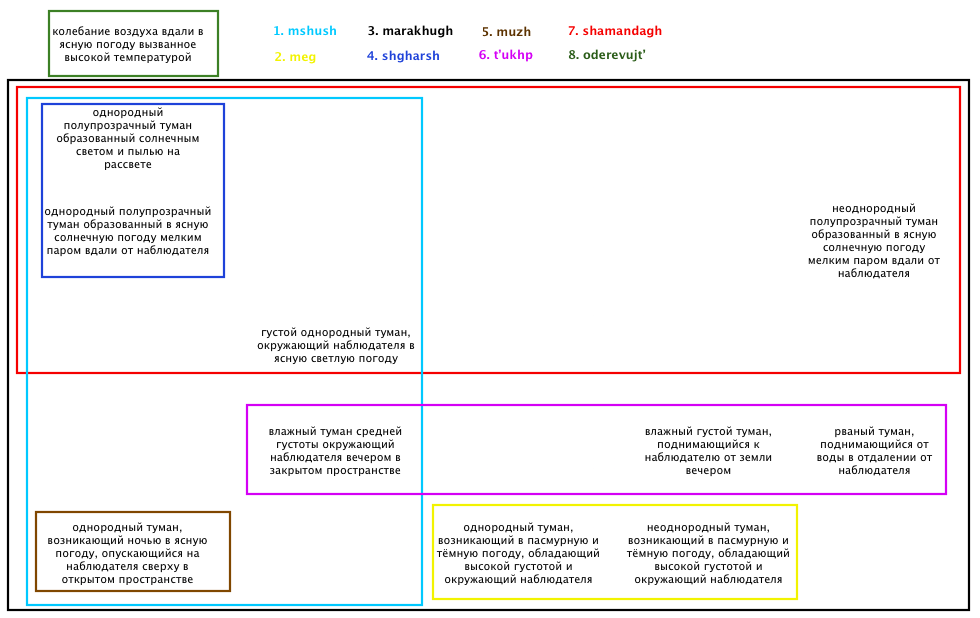
\includegraphics[width=\textwidth]{maps/ARMsemap.png}
    \caption{Карта семантического поля 'туман' для армянского языка}
    \label{fig:ARM}
\end{figure}

\bigskip

\begin{figure}[H]
    \centering
    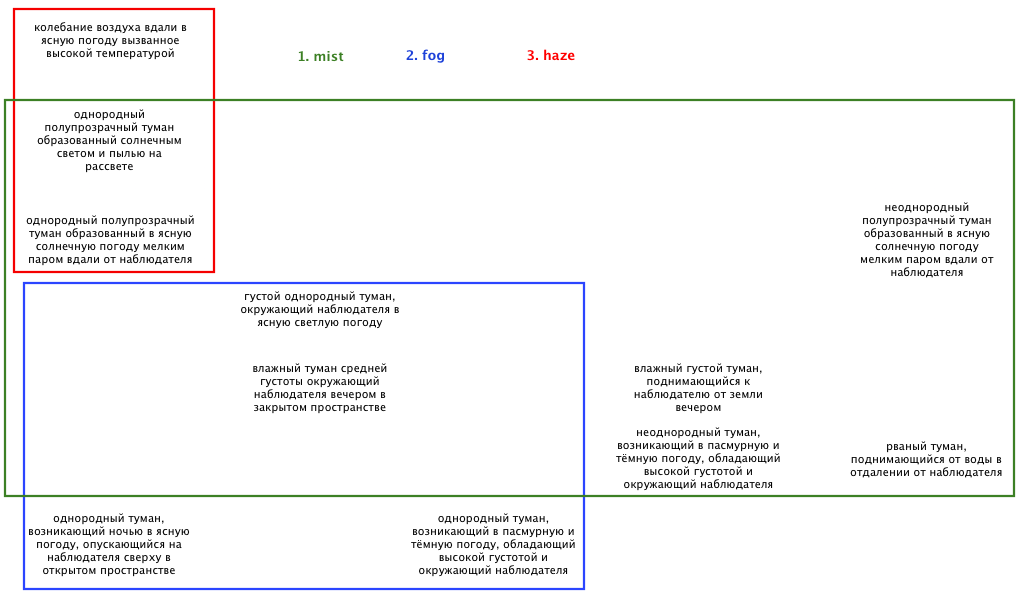
\includegraphics[width=\textwidth]{maps/ENsemap.png}
    \caption{Карта семантического поля 'туман' для английского языка}
    \label{fig:EN}
\end{figure}

\begin{figure}[H]
    \centering
    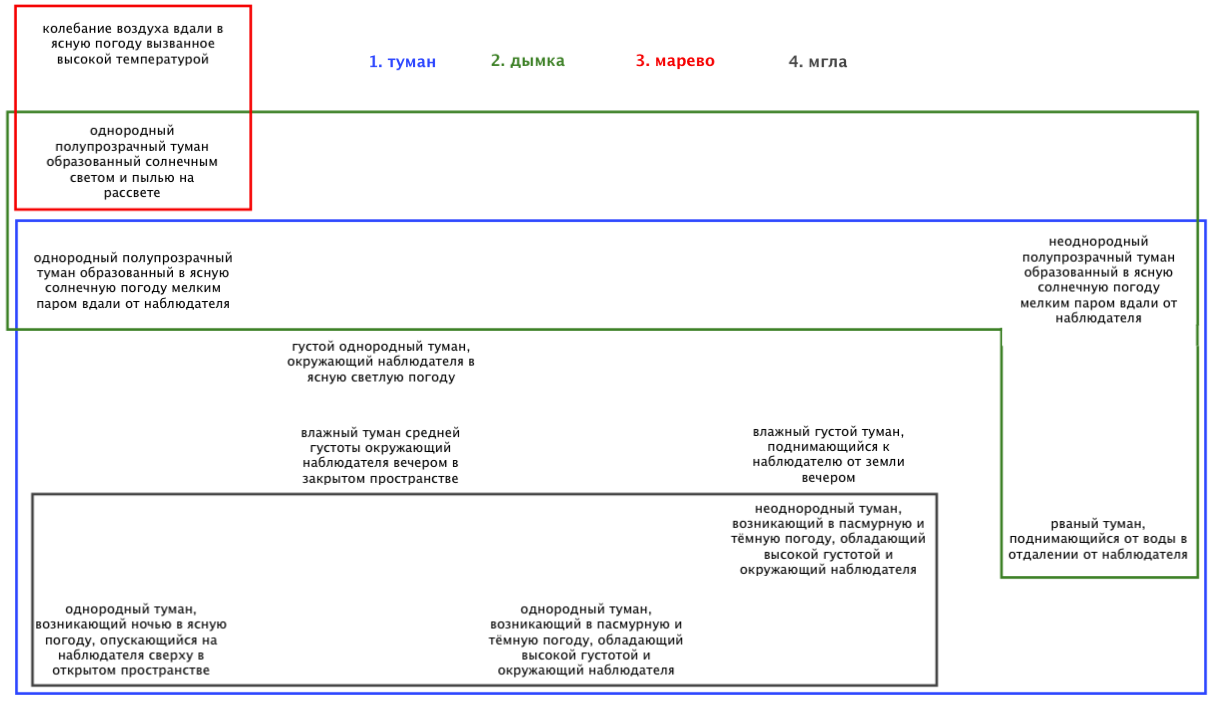
\includegraphics[width=\textwidth]{maps/RUsemap.png}
    \caption{Карта семантического поля 'туман' для русского языка}
    \label{fig:RU}
\end{figure}

\par Если сопоставить представленные здесь карты с информацией, обсуждавшейся ранее, можно обнаружить, что изображение лексем на карте сопровождается достаточно серьёзным огрублением, в том или ином виде свойственным любому типологическому исследованию. Однако главное --- карты не противоречат реальной языковой ситуации. Проблема огрубления во фреймовом подходе обсуждается в разделе \ref{final2}


\section{Заключение} \label{final}

\subsection{Результаты и перспективы исследования}

\par Подводя итоги, можно сказать, что проведённое нами исследование имеет достаточно большой потенциал для развития. Помимо близости семантического поля 'туман' к полям 'пар' и 'облако' на материале немецкого языка была также обнаружена близость с полем 'запах'. Лексико-типологическое исследование связей этих полей может оказаться весьма продуктивным.

\par Набор фреймов, относящихся к полю 'туман' значительно расширился и уточнился по сравнению с вариантом, представленным в \citep{соколовский2017}. Удалось изучить, в каком отношении состоят русские лексемы \textit{туман, дымка, марево} и \textit{мгла} как между собой, так и с их общепринятыми переводами на английский, немецкий и армянский языки. Описание богатого армянского поля теперь можно считать полным.

\par Интересным выводом стала и ошибочность или, по крайней мере, неподтверждённость гипотезы, сформулированной в разделе \ref{preview}. В каратинском, который можно отнести к горным языкам, было обнаружено рекордно малое количество лексикализаций, относящихся к полю 'туман'. В грузинском поверхностный анализ (продемонстрировавший исключительное богатство армянских лексикализаций в \citep{соколовский2017}) дал лишь базовый набор из двух лексем. В связи с этим можно предположить, что глубокий анализ с привлечением максимального количества ресурсов выявит количество релевантных лексем, не превышающее оного в русском или же английском языках.

\par Наконец, еще одно потенциальное направление, в котором может быть продолжена эта работа, - это подробный анализ семантического поля 'туман' в финском языке. Кроме того, естественным развитием данного исследования может стать расширение выборки языков.

\subsection{К вопросу огрубления в лексико-типологическом исследовании} \label{final2}

\par Любое типологическое исследование сталкивается на определённом этапе с проблемой огрубления. Примерно равные языковые единицы воспринимаются как абсолютно равные, с целью формирования общей картины, в которой у каждого языка и у каждой языковой единицы есть своё определённое место. Проблема становится острее с увеличением абстрактности рассматриваемых единиц. 

\par Фреймовый подход к лексической типологии --- это метод огрубления данных о лексическом разнообразии. Он чрезвычайно эффективен и может весьма быстро показать базовые семантические связи. Его применение в глагольных полях оправданно, т.к. глагол даёт возможность выделять фреймы по ограничениям, накладываемым на субъект и других участников ситуации. Его применение в признаковых полях тоже оправдано - и по той же причине . Иными словами, фреймовый подход оправдан в тех случаях, когда дистрибутивные методы могут продемонстрировать относительную точность. 

\par В именных полях ситуация обстоит сложнее. Как было сказано в разделе \ref{preview}, не так очевидно, какая именно сочетаемость существительного играет ключевую роль. Потому дистрибутивные методы демонстрируют здесь меньшую точность. Набор фреймов, выделенных вручную, носит более условный характер.

\par Большая часть элементов поля, рассматривавшегося в нашем исследовании, продуктивно метафоризуются. Метафорические значения не включаются в семантические карты, однако вопрос проведения чёткой границы между прямым и метафорическим значением тоже нельзя назвать закрытым. В нашем поле метафорическое значение лексемы может оказаться базовым. Именные поля природных явлений и, к примеру, оболочек объектов --- это совершенно непохожие по своему устройству области, а значит и методы, применяемые для их анализа, должны различаться. 

\par Иными словами, если лексический типолог исследует, например, поле оболочек объектов \citep{шкурныйвопрос}, он вынужден пренебрегать некоторыми небольшими семантическими компонентами рассматриваемых лексем (что, например, корка апельсина чаще сухая, а кожура свежая). Это что-то несущественное, и для нанесения лексемы на семантическую карту подобные факты непринципиальны. Однако в исследовании семантического поля какого-нибудь природного явления для нанесения лексемы на двумерный фрейм исследователь вынужден пренебрегать более значительной долей семантики. То, что армянскими лексемами \textit{meg} и \textit{muzh} может называться довольно широкий спектр различных туманов в зависимости от того, какое чувство они вызывают (страх для \textit{meg} или тяжесть \textit{muzh}), не отражено и не может быть отражено в рамках фреймового подхода.


\pagebreak
\section{Литература}
\renewcommand{\bibsection}{}
\bibliographystyle{ugost2008ns.bst}
\bibliography{bibliography.bib} 

\section{Онлайн ресурсы}

\noindent \hypertarget{eanc}{Восточноармянский национальный корпус (ВАНК)}:\;
\url{http://www.eanc.net} \medskip

\noindent \hypertarget{tenten}{Корпуса ruTenTen$11$, deTenTen$13$, enTenTen$15$ и BNC  на базе Sketch Engine}:\\ \url{https://app.sketchengine.eu} \medskip

\noindent \hypertarget{glosbe}{Многоязычный онлайн словарь Glosbe}:\;
\url{https://ru.glosbe.com} \medskip

\noindent \hypertarget{ruscorpora}{Национальный корпус русского языка (НКРЯ)}:\;
\url{http://ruscorpora.ru} \medskip

\noindent \hypertarget{gt}{Переводчик Google}:\; \url{https://translate.google.com} \medskip

\noindent \hypertarget{yt}{Переводчик Yandex}:\; \url{https://translate.yandex.com} \medskip


\noindent \hypertarget{inst}{Поиск по хэштегам в сети Instagram}:\; 
\url{https://twitnow.ru/instagram} \medskip

\noindent \hypertarget{mlext}{Проект московская лексикотипологическая группа (MLexT)}:\; 
\url{http://lextyp.org} \medskip

\noindent \hypertarget{github}{Проект страницы опроса на Github}:\; 
\url{https://github.com/sukalov/lingform} \medskip

\noindent \hypertarget{rusvectores}{Семантические модели для русского языка RusVectōrēs}:\;
\url{https://rusvectores.org/ru} \medskip

\noindent Словари и энциклопедии на Академике:\; 
\url{https://dic.academic.ru} \medskip

\noindent \hypertarget{form}{Страница с опросом}:\; 
\url{https://lingform.herokuapp.com}\medskip


\pagebreak
\section{Приложение} \label{приложение}
    
\begin{figure}[H]
    \centering
    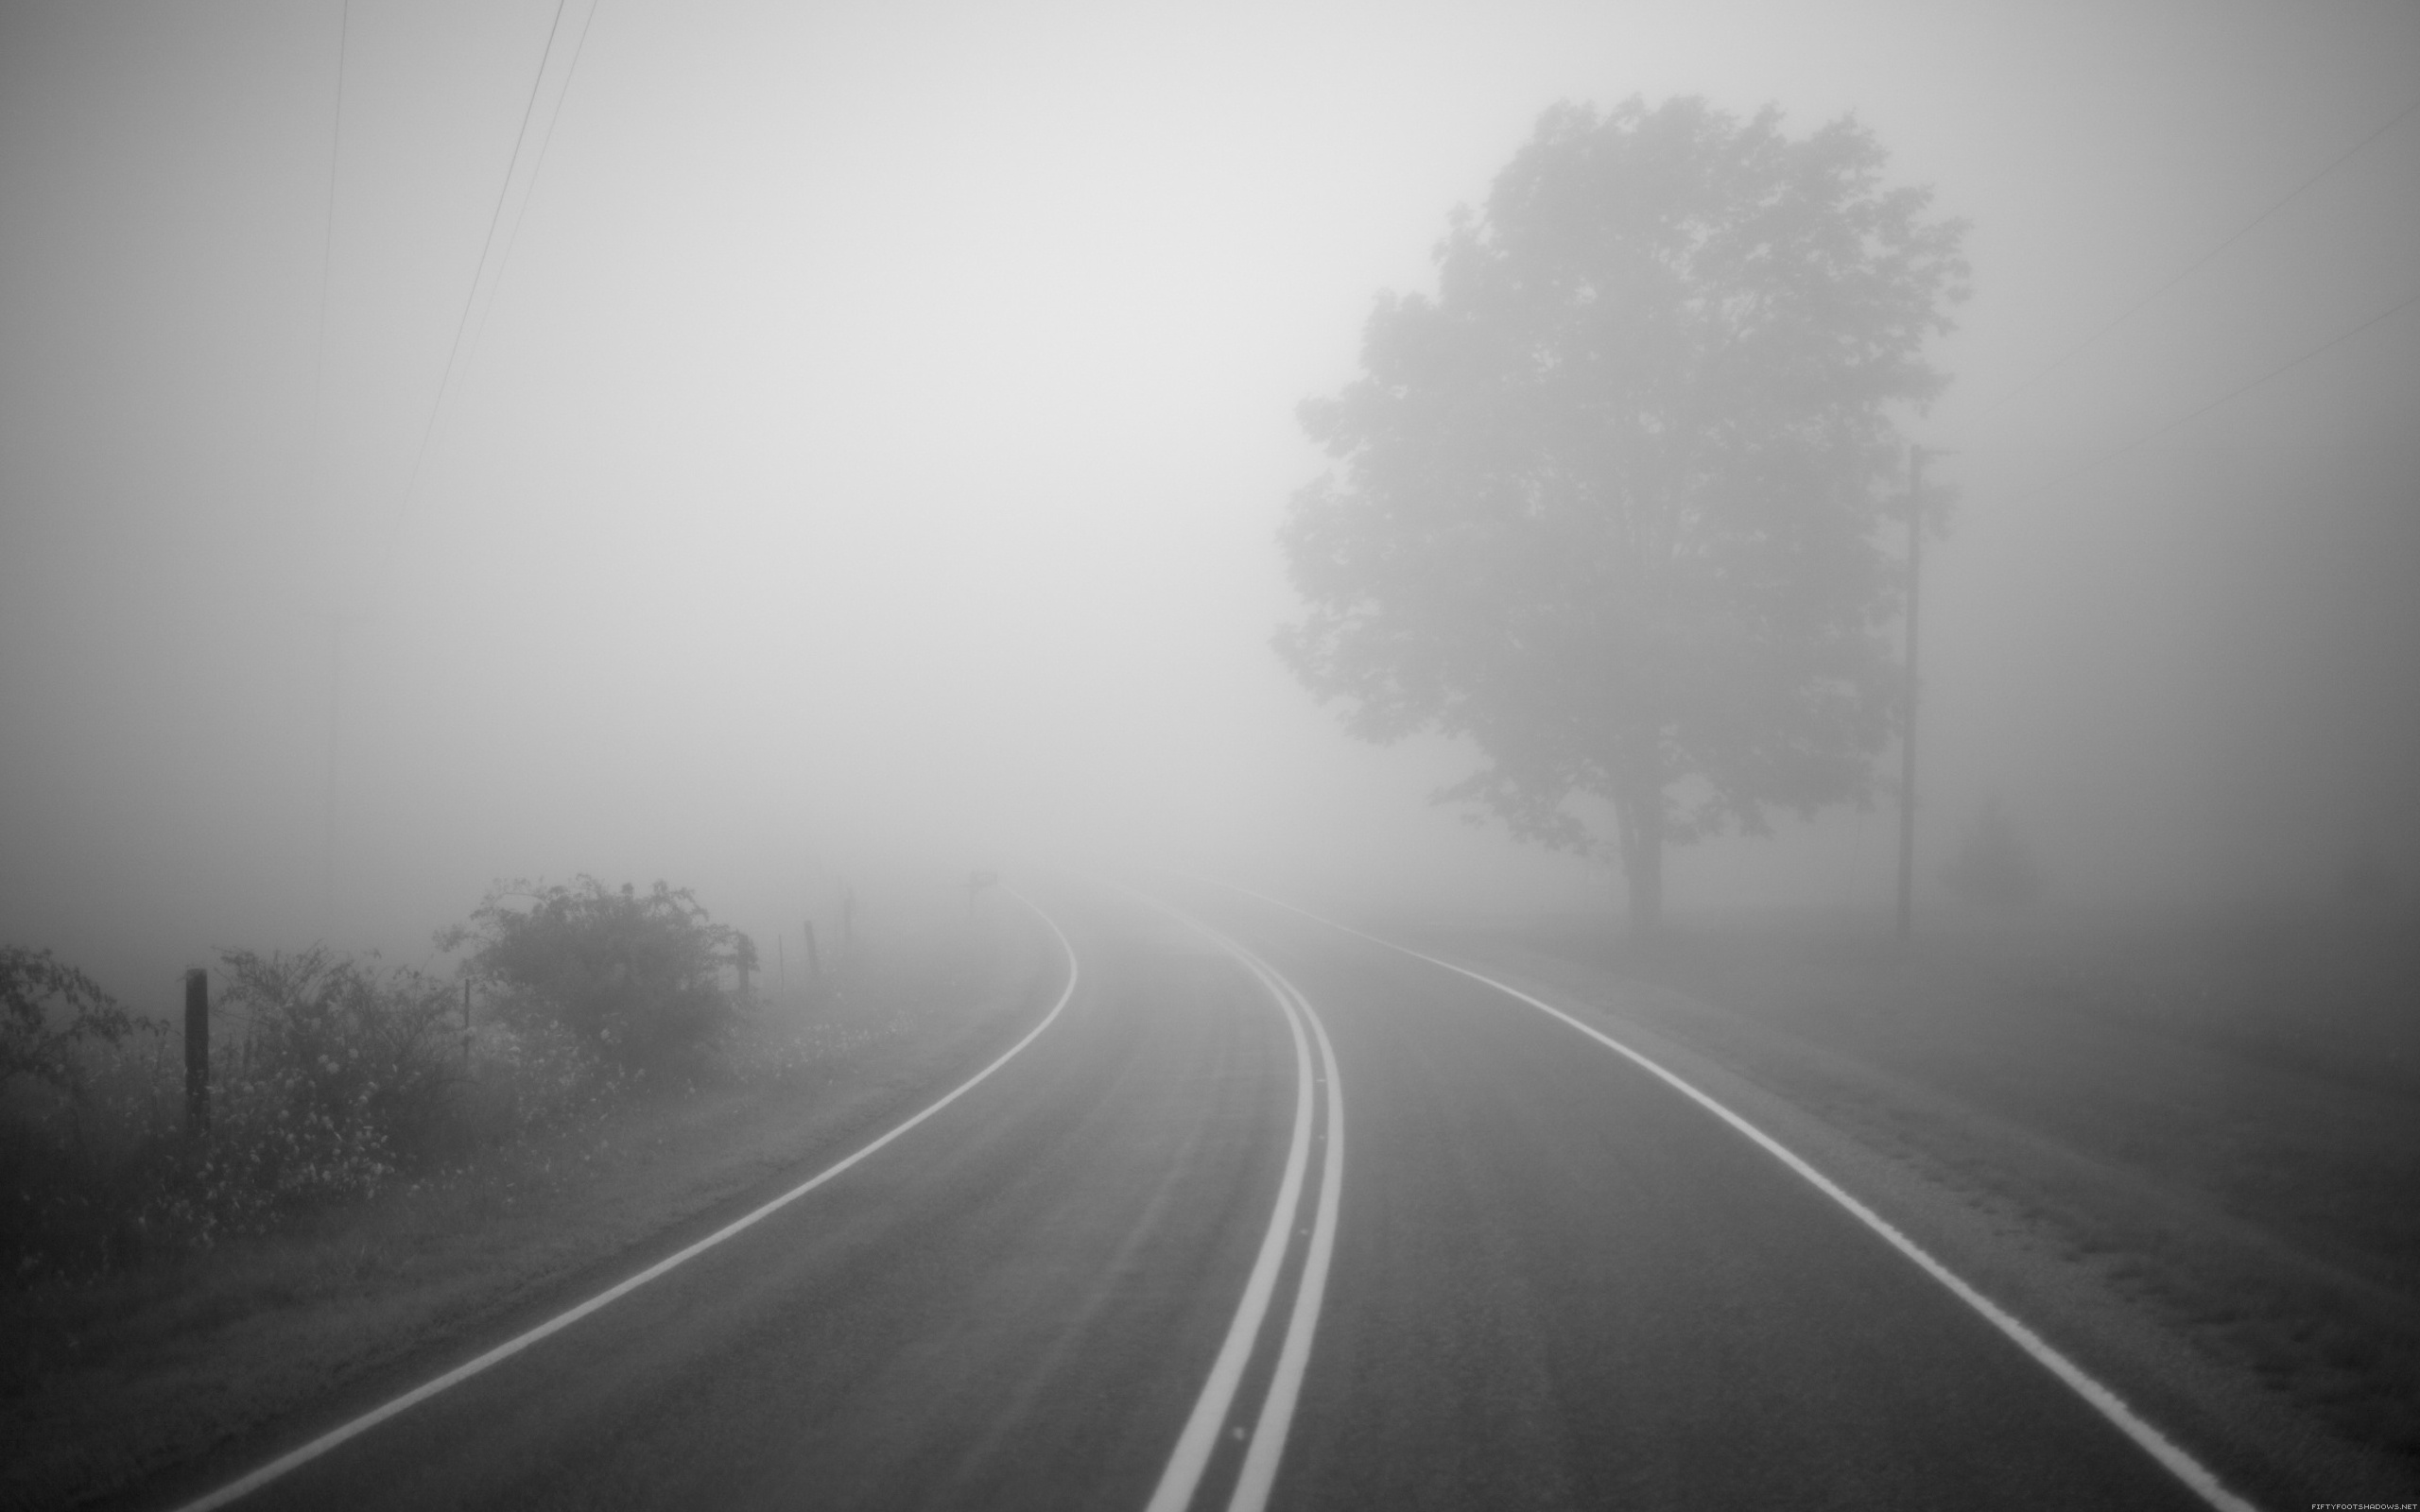
\includegraphics[width=\linewidth]{fogs/fog01.jpg} 
    \caption{}
    \label{fig:r1}
\end{figure}

\begin{figure}[H]
    \centering
    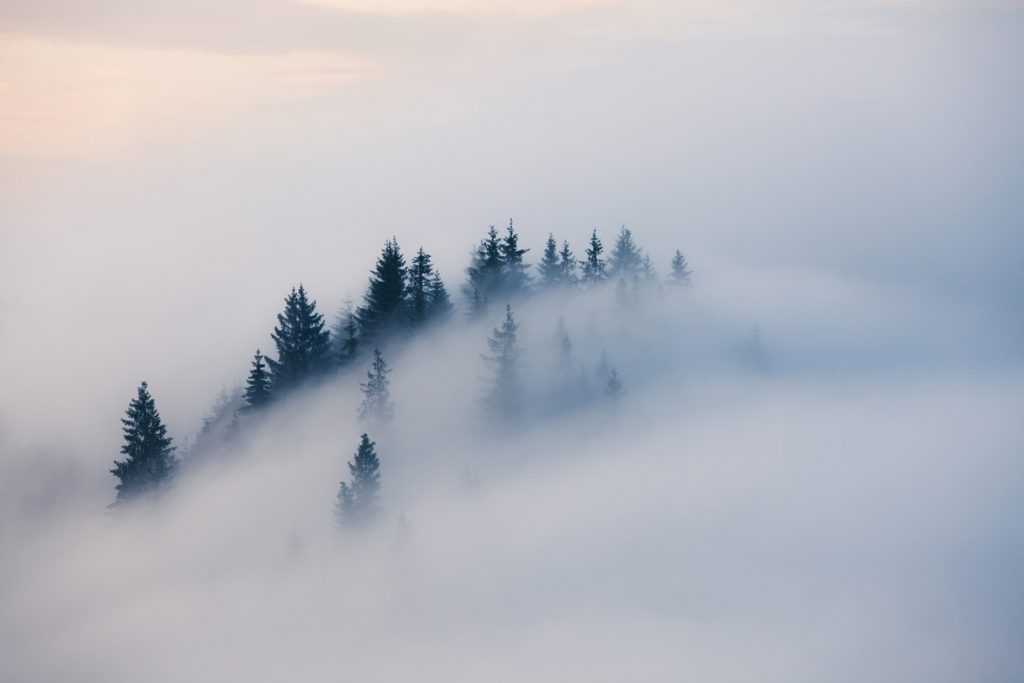
\includegraphics[width=\linewidth]{fogs/fog02.jpg} 
    \caption{}
    \label{fig:r2}
\end{figure}

\begin{figure}[H]
    \centering
    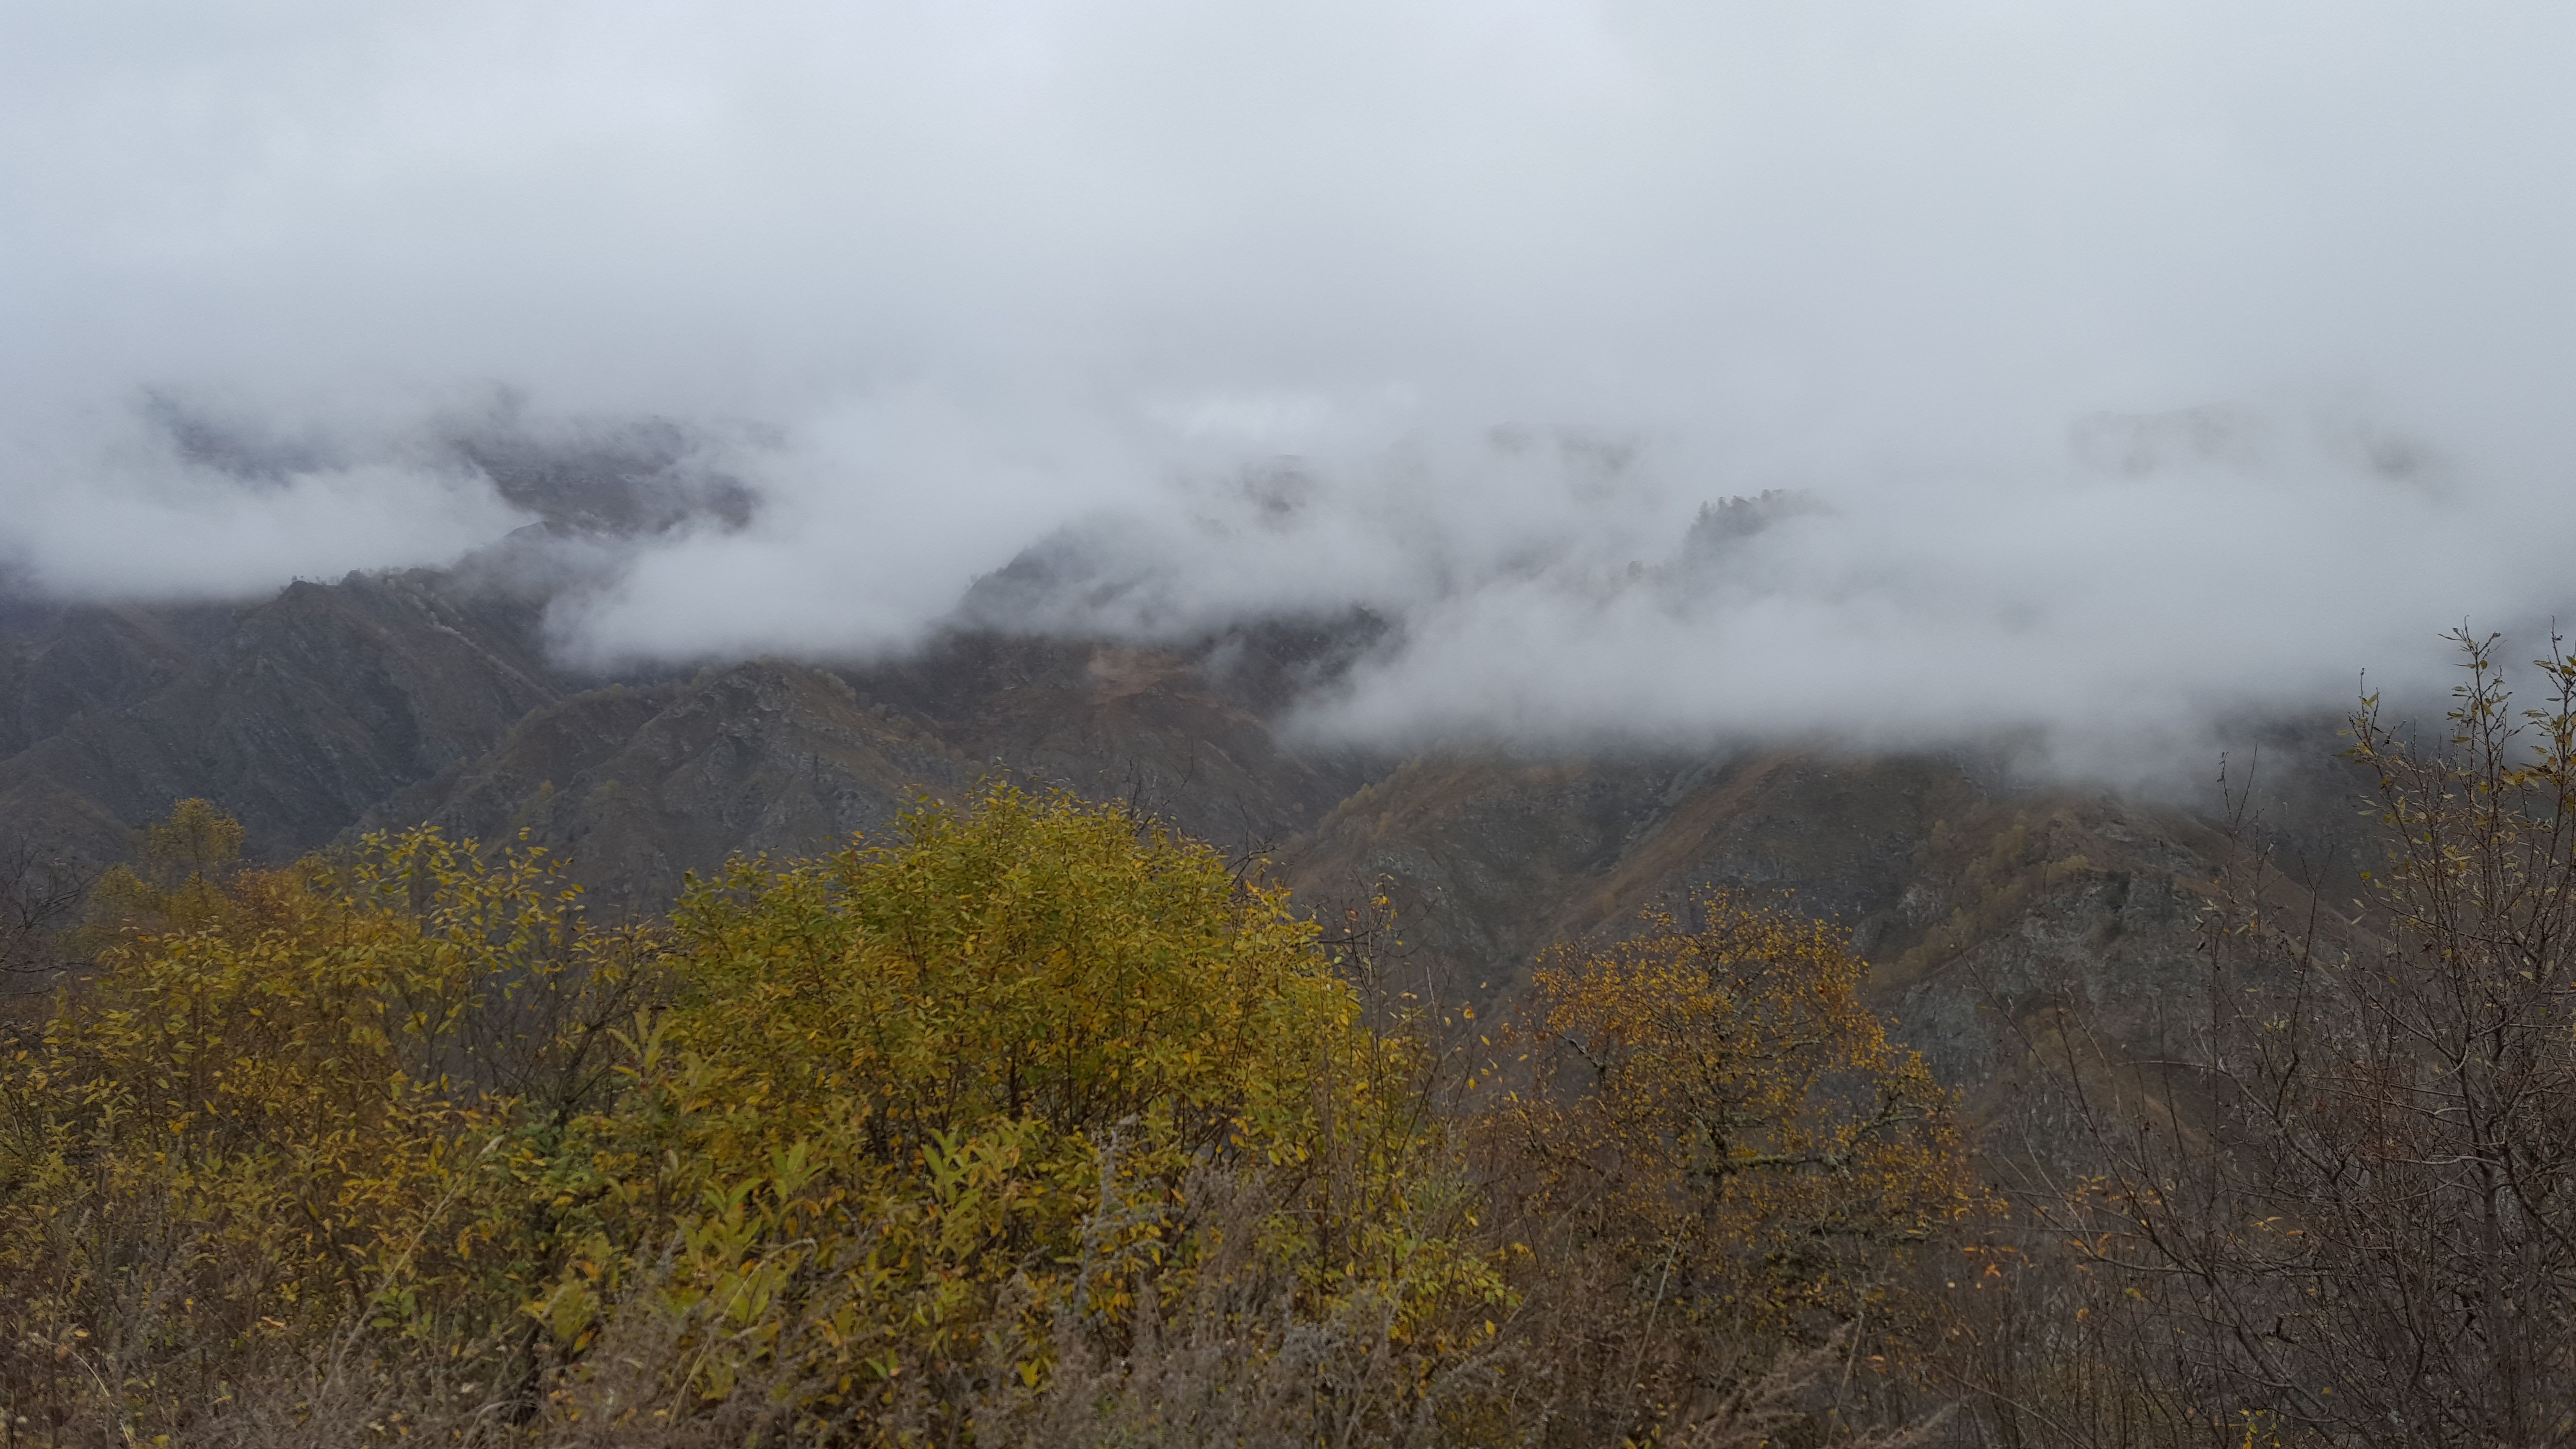
\includegraphics[width=\linewidth]{fogs/fog03.jpg} 
    \caption{}
    \label{fig:r3}
\end{figure}

\begin{figure}[H]
    \centering
    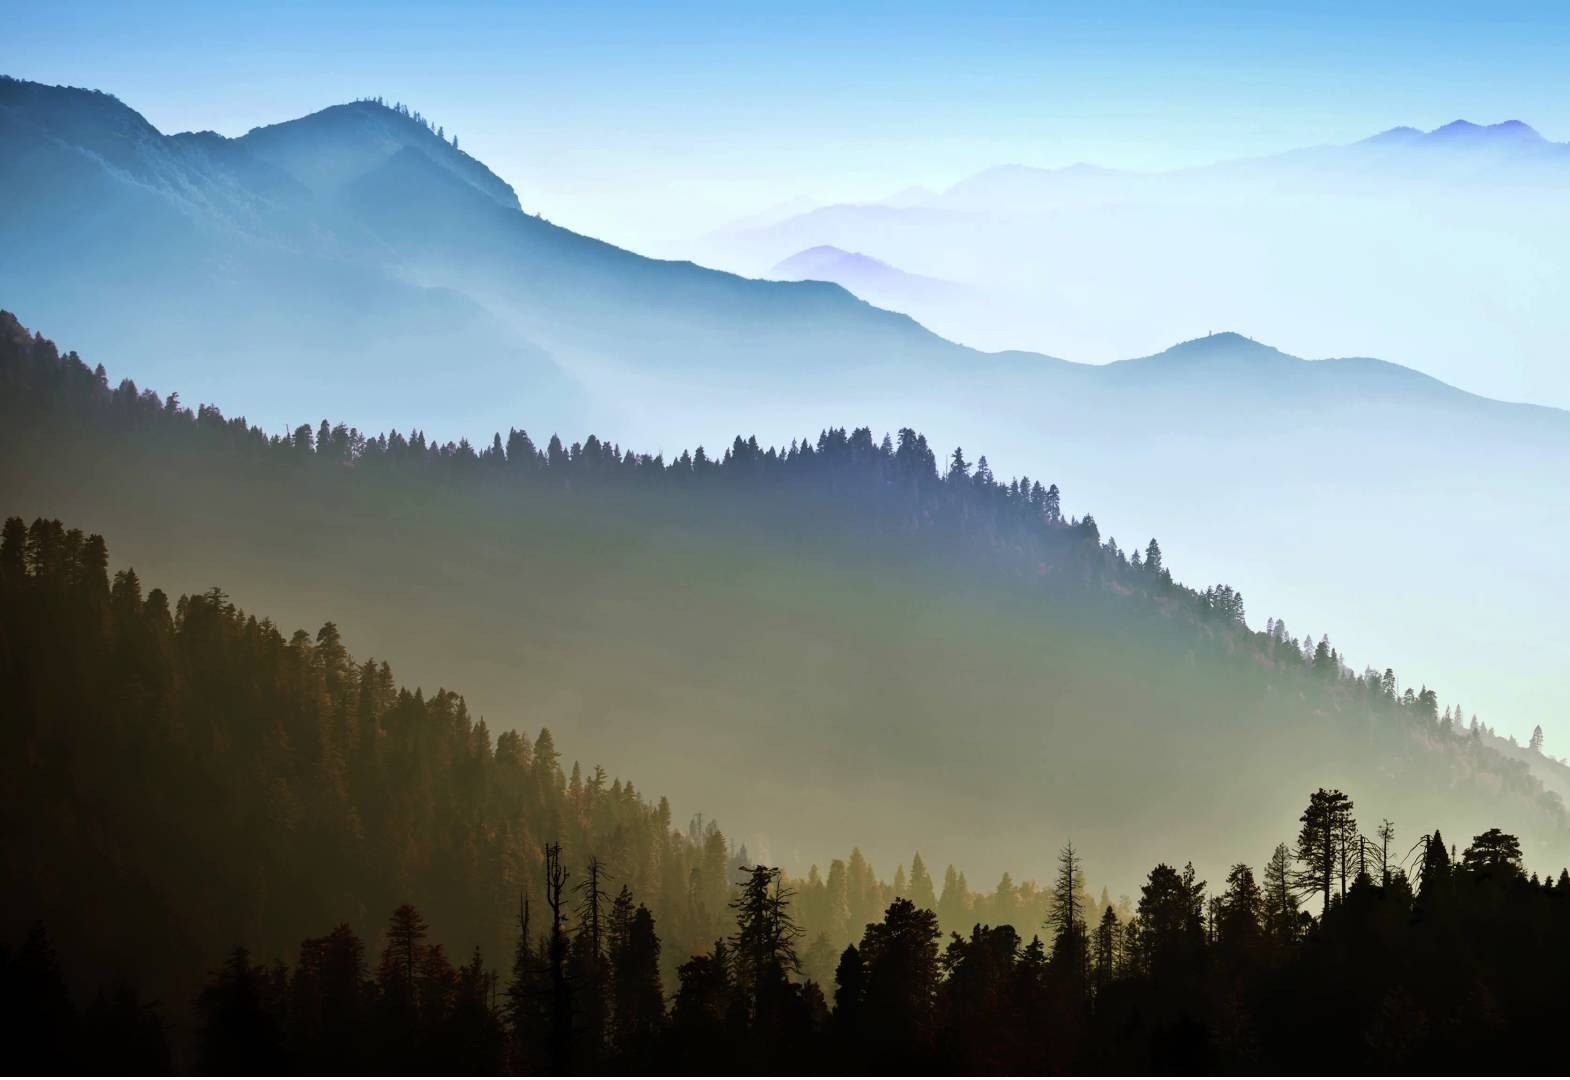
\includegraphics[width=\linewidth]{fogs/fog04.jpg} 
    \caption{}
    \label{fig:r4}
\end{figure}

\begin{figure}[H]
    \centering
    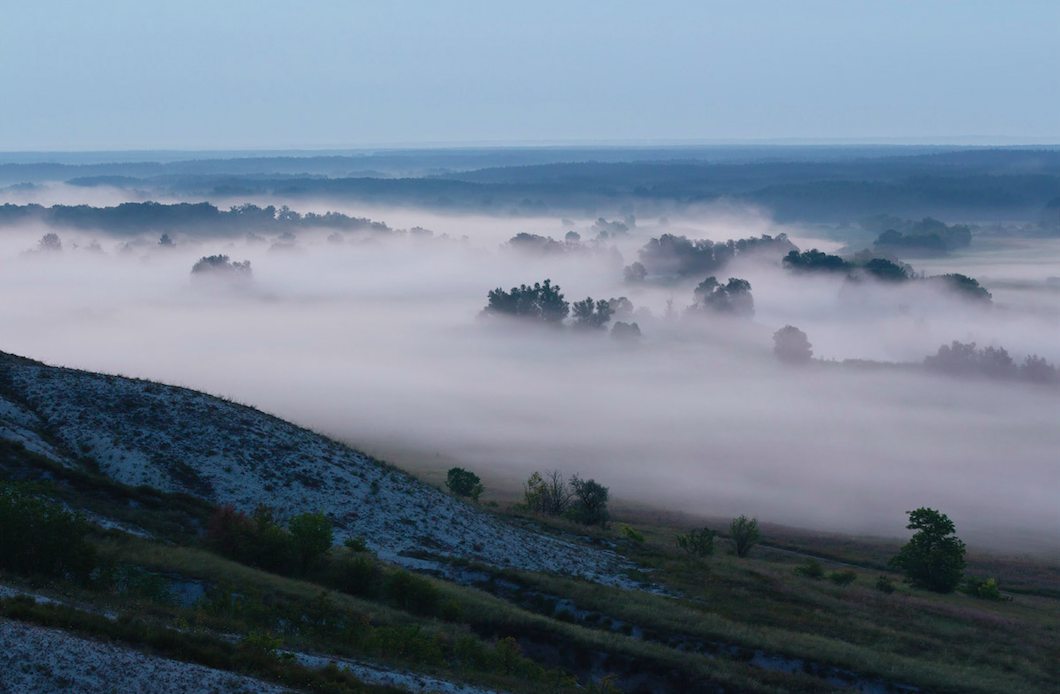
\includegraphics[width=\linewidth]{fogs/fog05.jpg} 
    \caption{}
    \label{fig:r5}
\end{figure}

\begin{figure}[H]
    \centering
    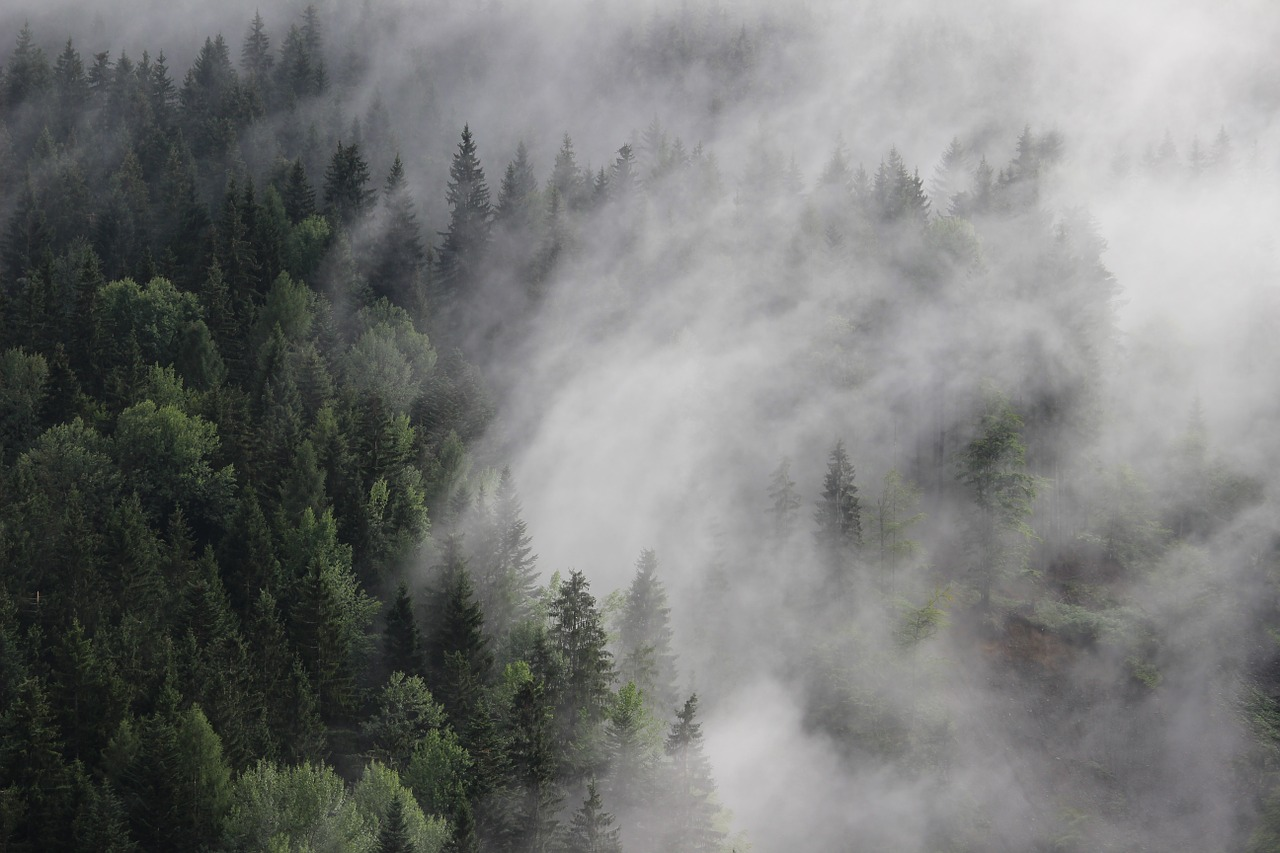
\includegraphics[width=\linewidth]{fogs/fog06.jpg} 
    \caption{}
    \label{fig:r6}
\end{figure}

\begin{figure}[H]
    \centering
    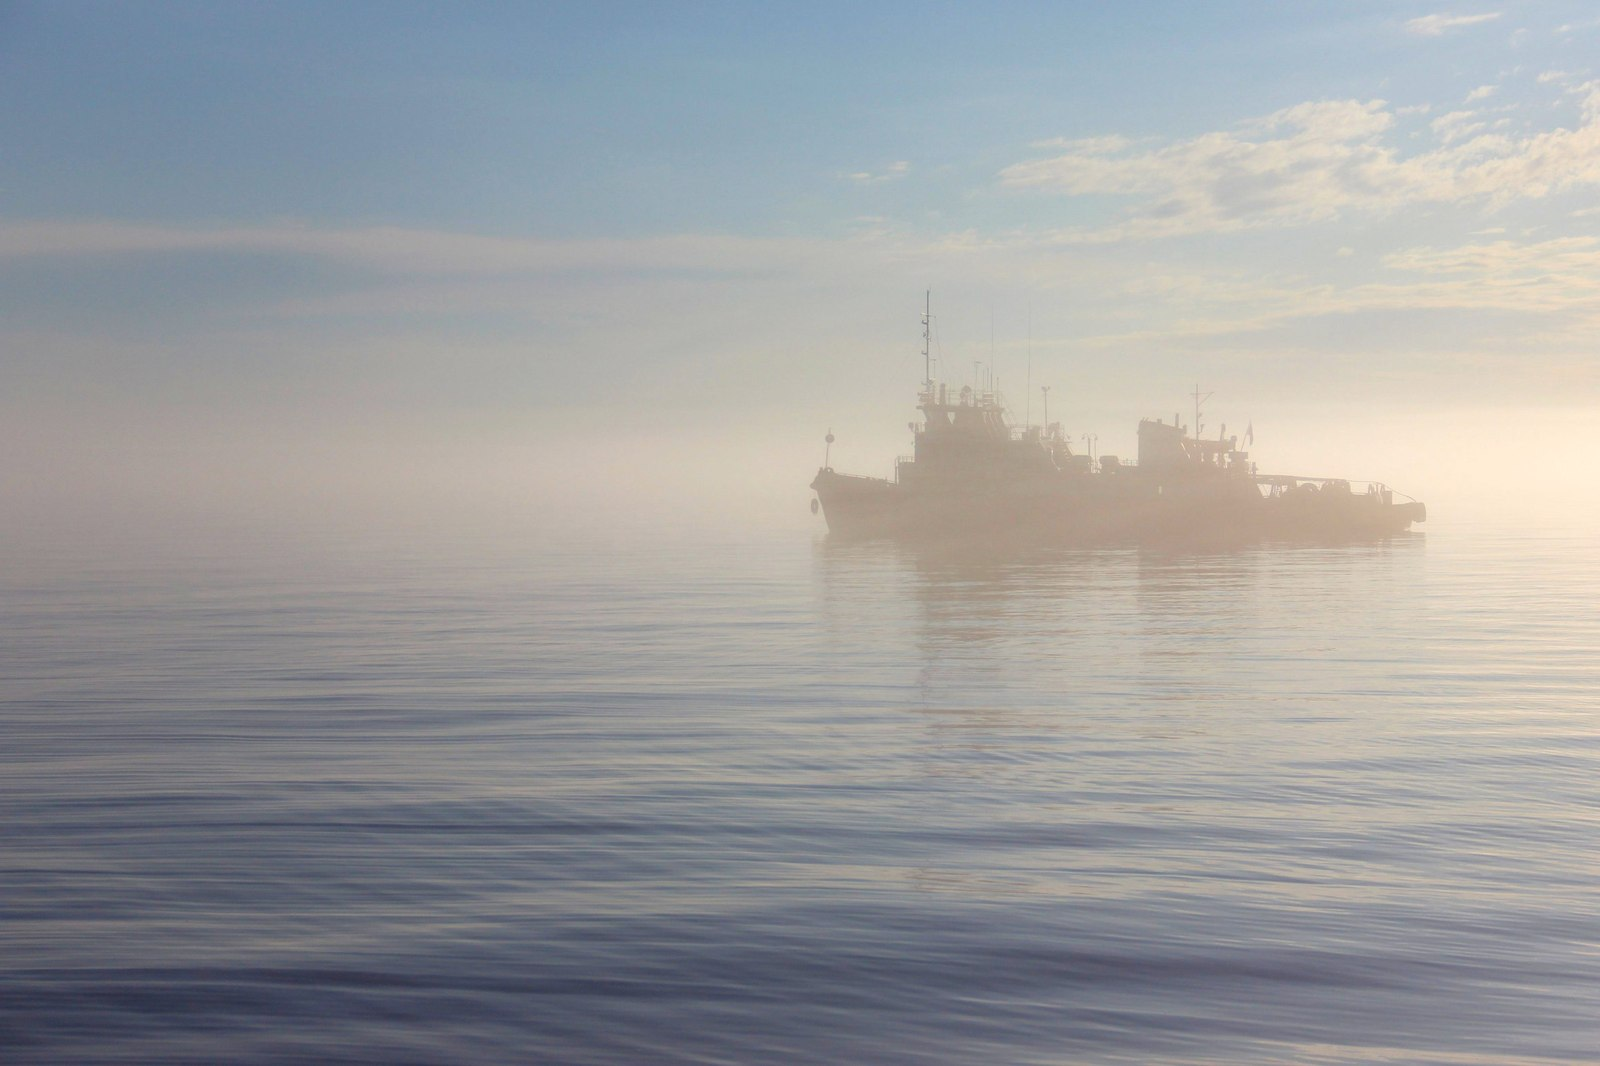
\includegraphics[width=\linewidth]{fogs/fog07.jpg} 
    \caption{}
    \label{fig:r7}
\end{figure}

\begin{figure}[H]
    \centering
    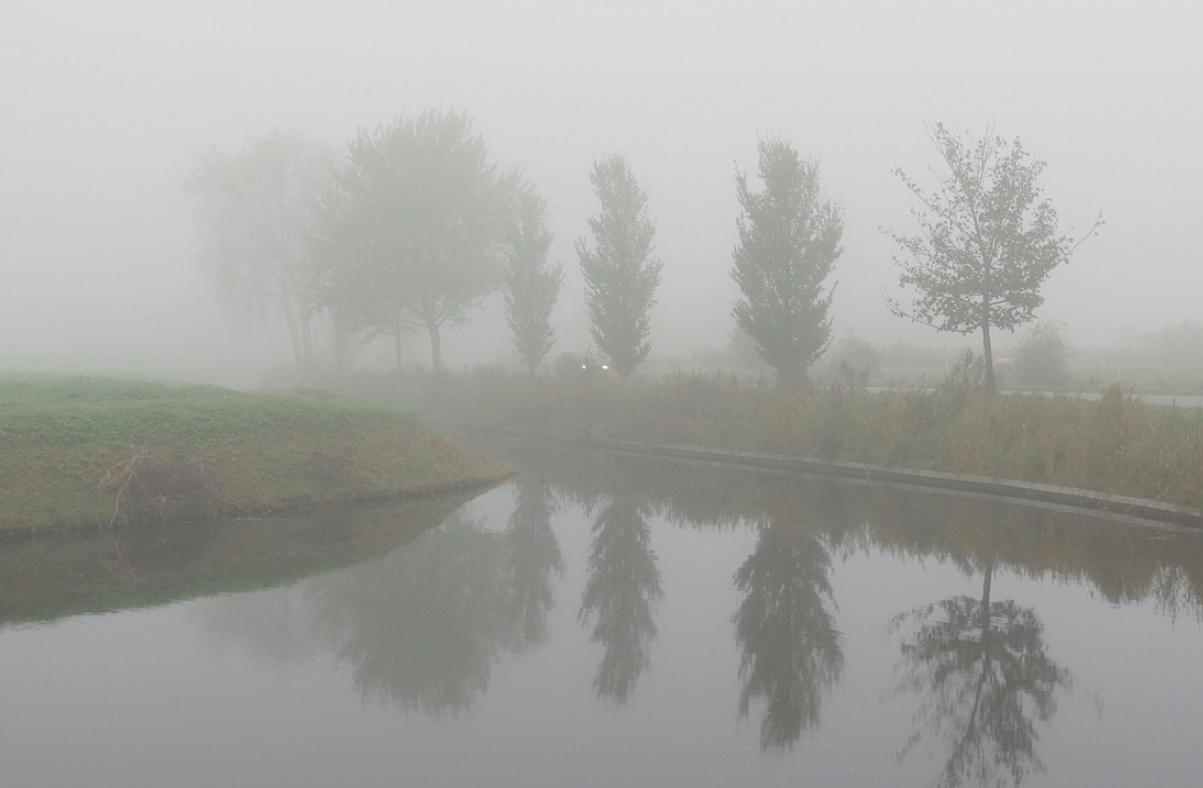
\includegraphics[width=\linewidth]{fogs/fog08.jpg} 
    \caption{}
    \label{fig:r8}
\end{figure}

\begin{figure}[H]
    \centering
    
\includegraphics[width=\linewidth]{fogs/fog09.jpg} 
    \caption{}
    \label{fig:r9}
\end{figure}

\begin{figure}[H]
    \centering
    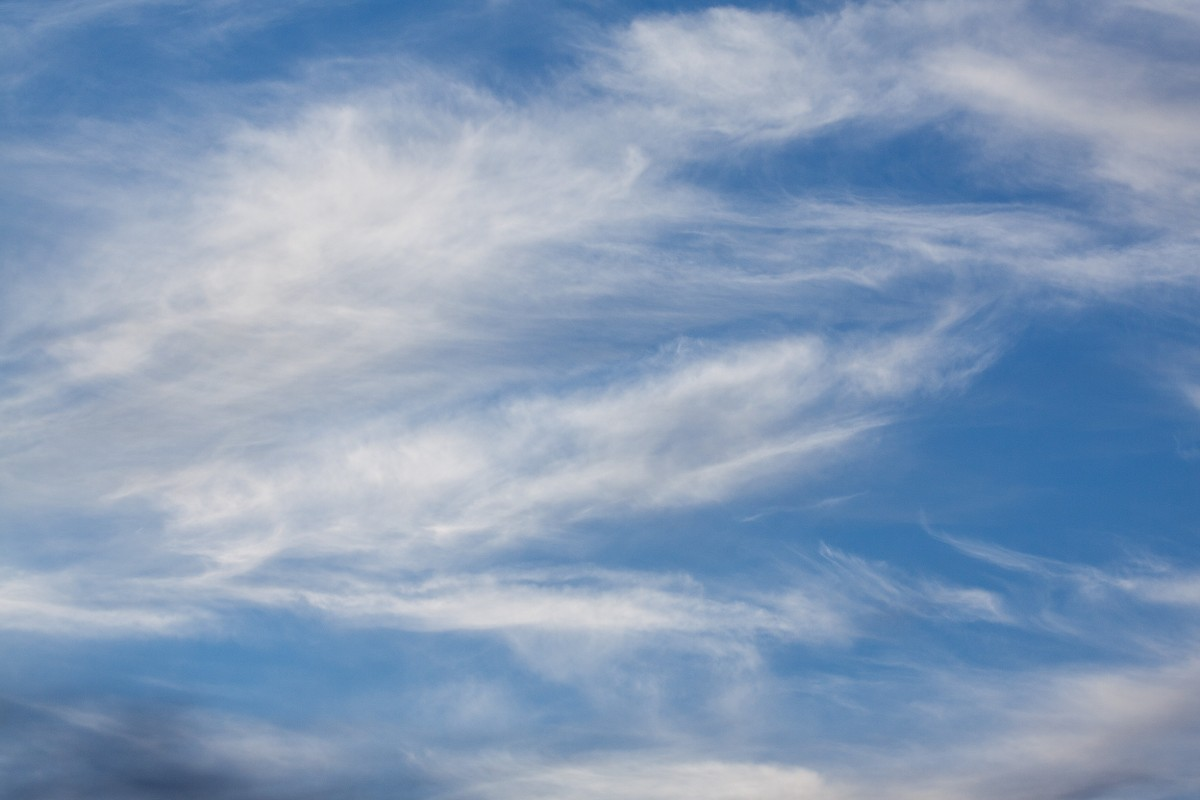
\includegraphics[width=\linewidth]{fogs/fog10.jpg} 
    \caption{}
    \label{fig:r10}
\end{figure}

\begin{figure}[H]
    \centering
    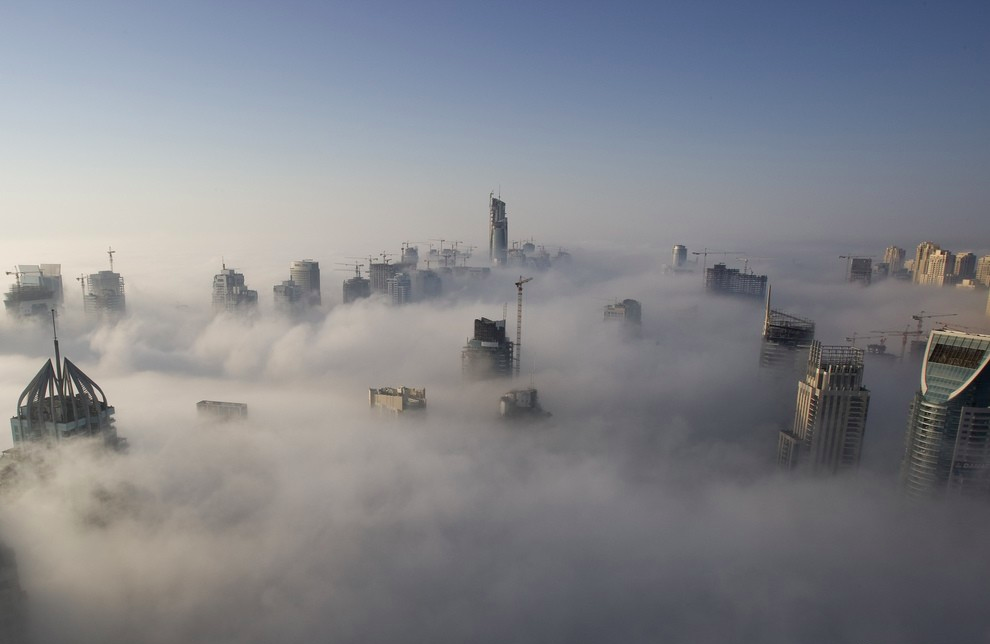
\includegraphics[width=\linewidth]{fogs/fog11.jpg} 
    \caption{}
    \label{fig:r11}
\end{figure}

\begin{figure}[H]
    \centering
    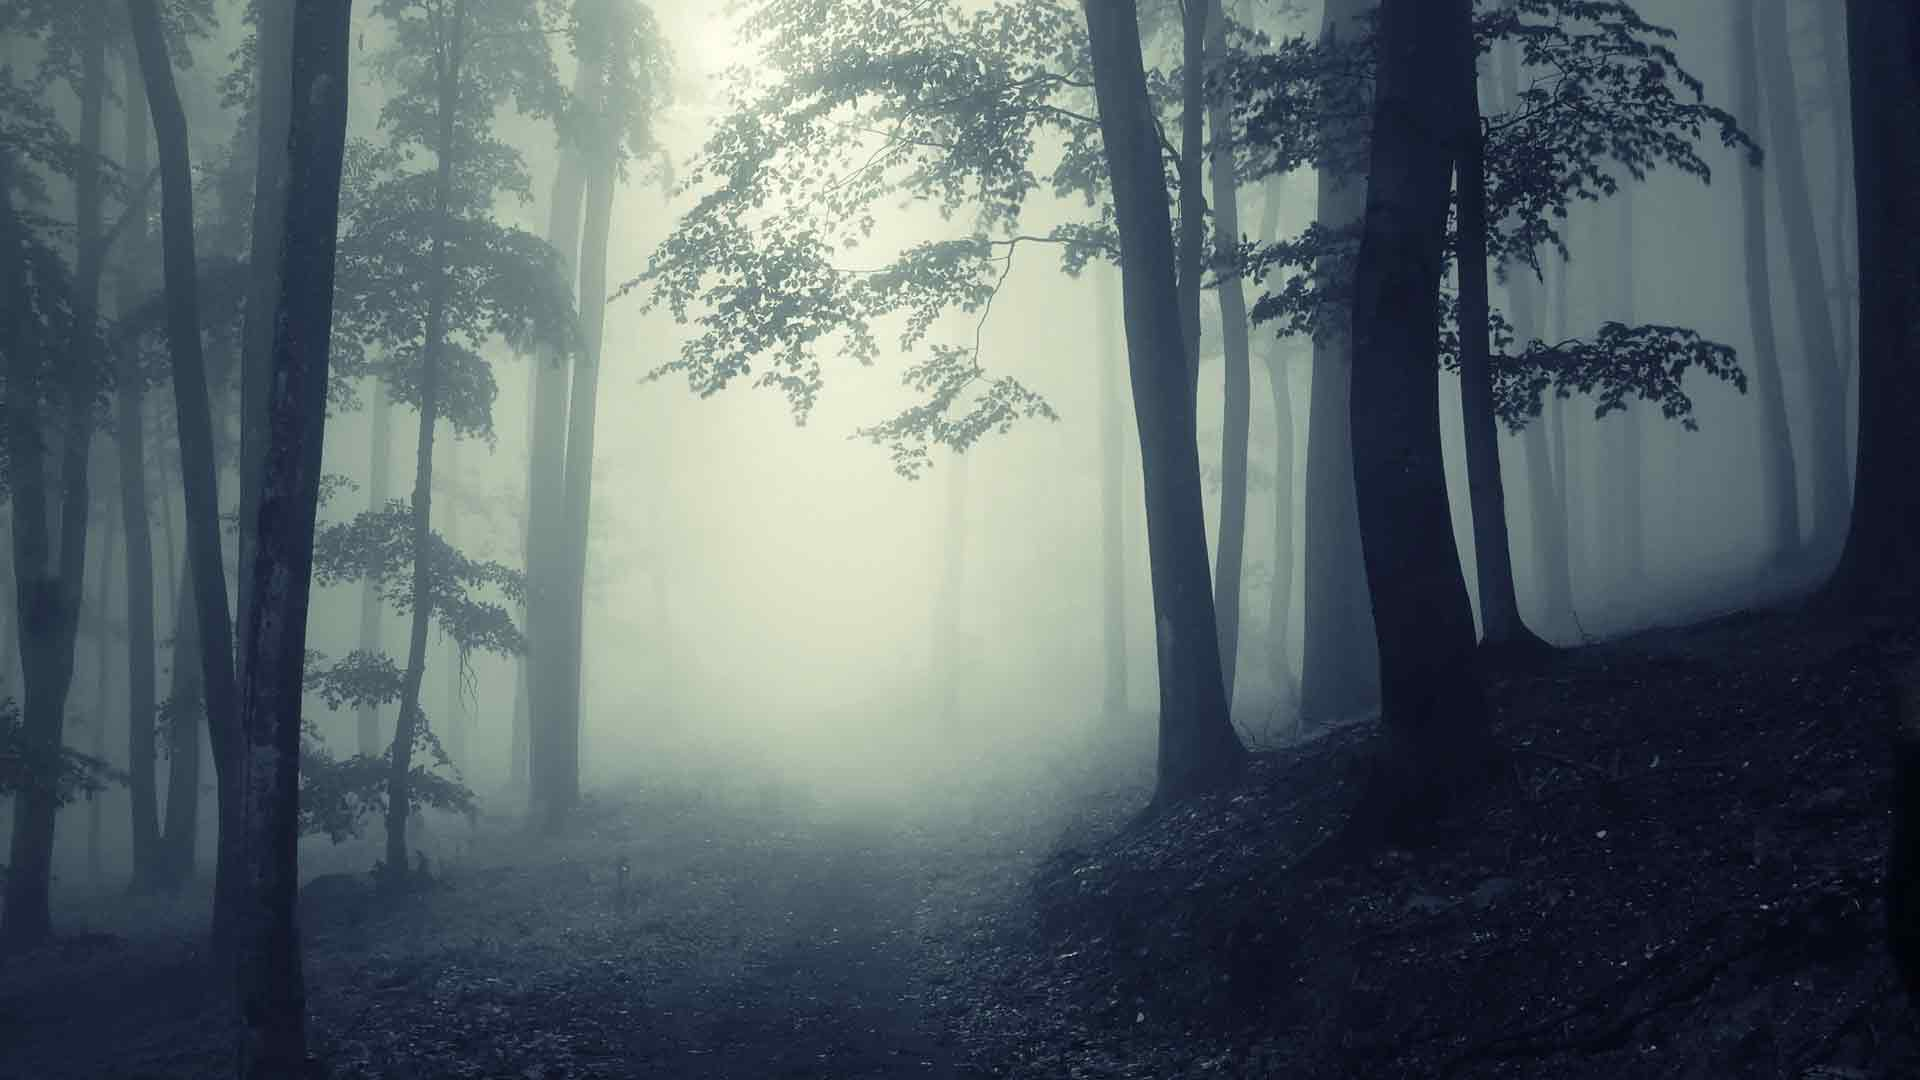
\includegraphics[width=\linewidth]{fogs/fog12.jpg} 
    \caption{}
    \label{fig:r12}
\end{figure}

\begin{figure}[H]
    \centering
    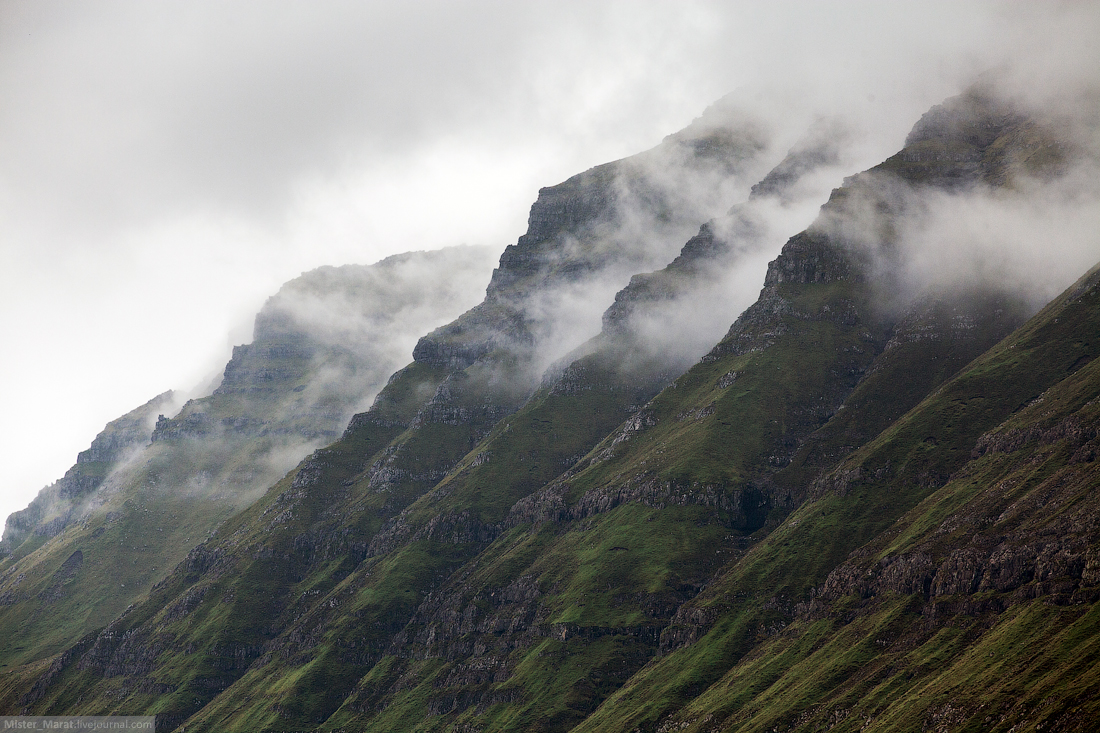
\includegraphics[width=\linewidth]{fogs/fog13.jpg} 
    \caption{}
    \label{fig:r13}
\end{figure}

\begin{figure}[H]
    \centering
    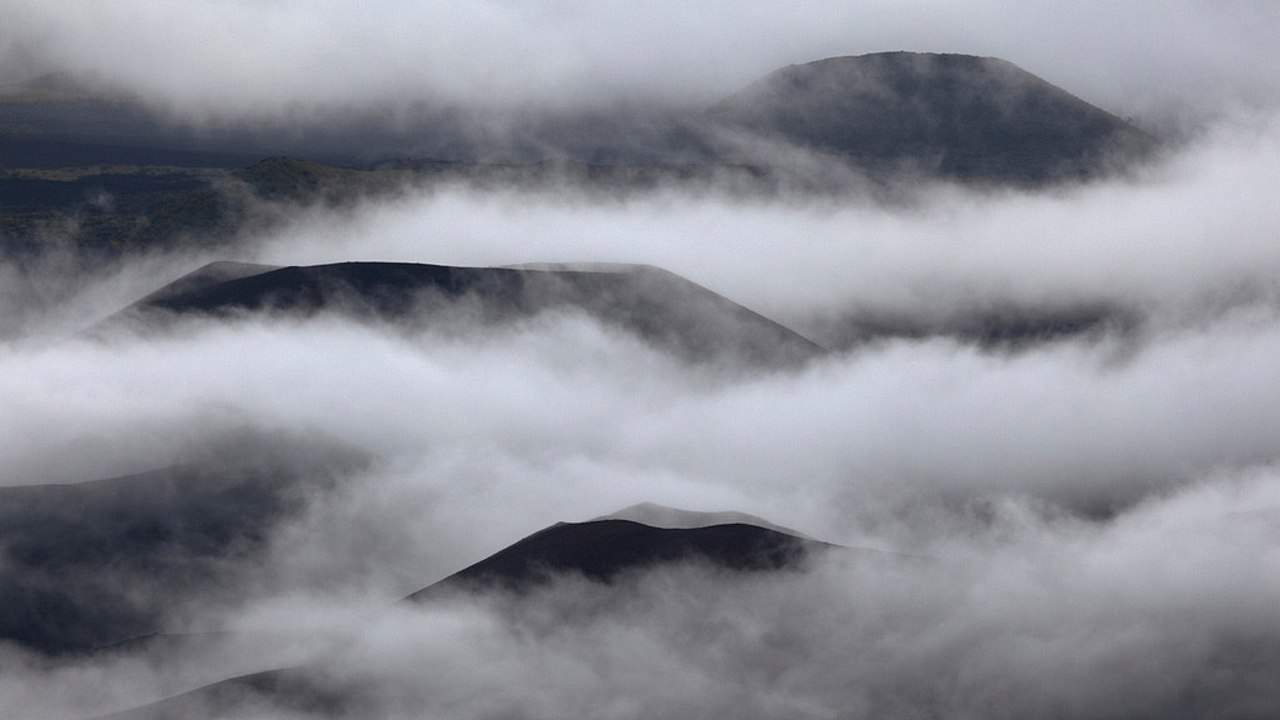
\includegraphics[width=\linewidth]{fogs/fog14.jpg} 
    \caption{}
    \label{fig:r14}
\end{figure}

\begin{figure}[H]
    \centering
    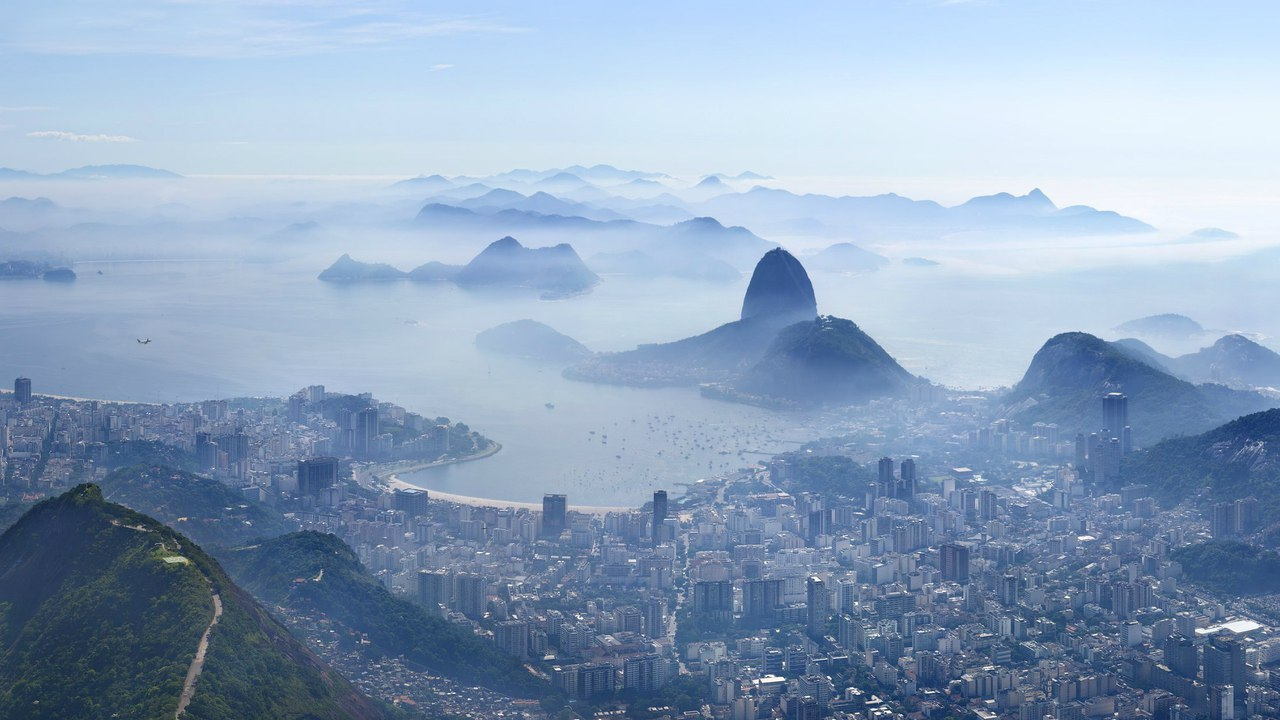
\includegraphics[width=\linewidth]{fogs/fog15.jpg} 
    \caption{}
    \label{fig:r15}
\end{figure}

\begin{figure}[H]
    \centering
    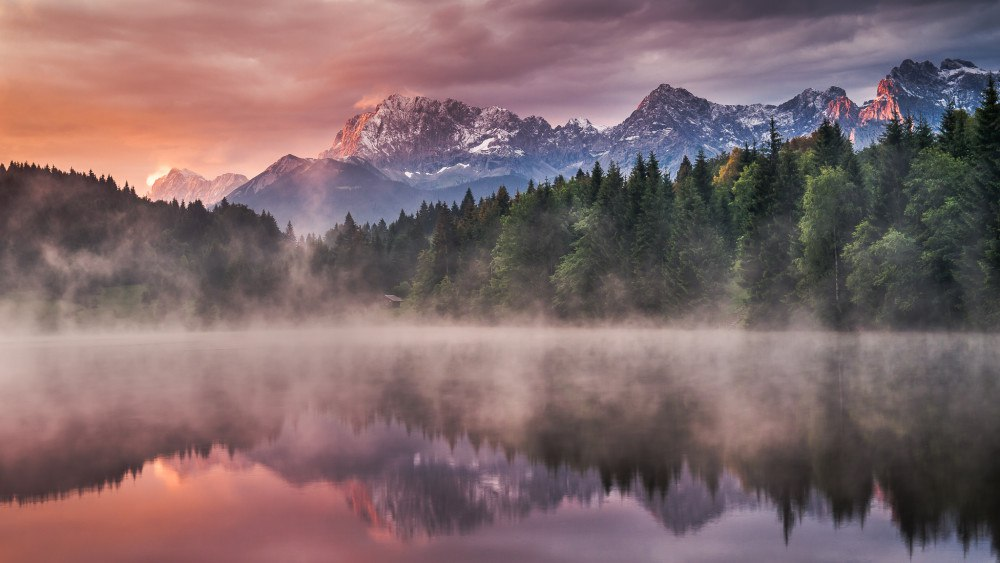
\includegraphics[width=\linewidth]{fogs/fog16.jpg} 
    \caption{}
    \label{fig:r16}
\end{figure}

\begin{figure}[H]
    \centering
    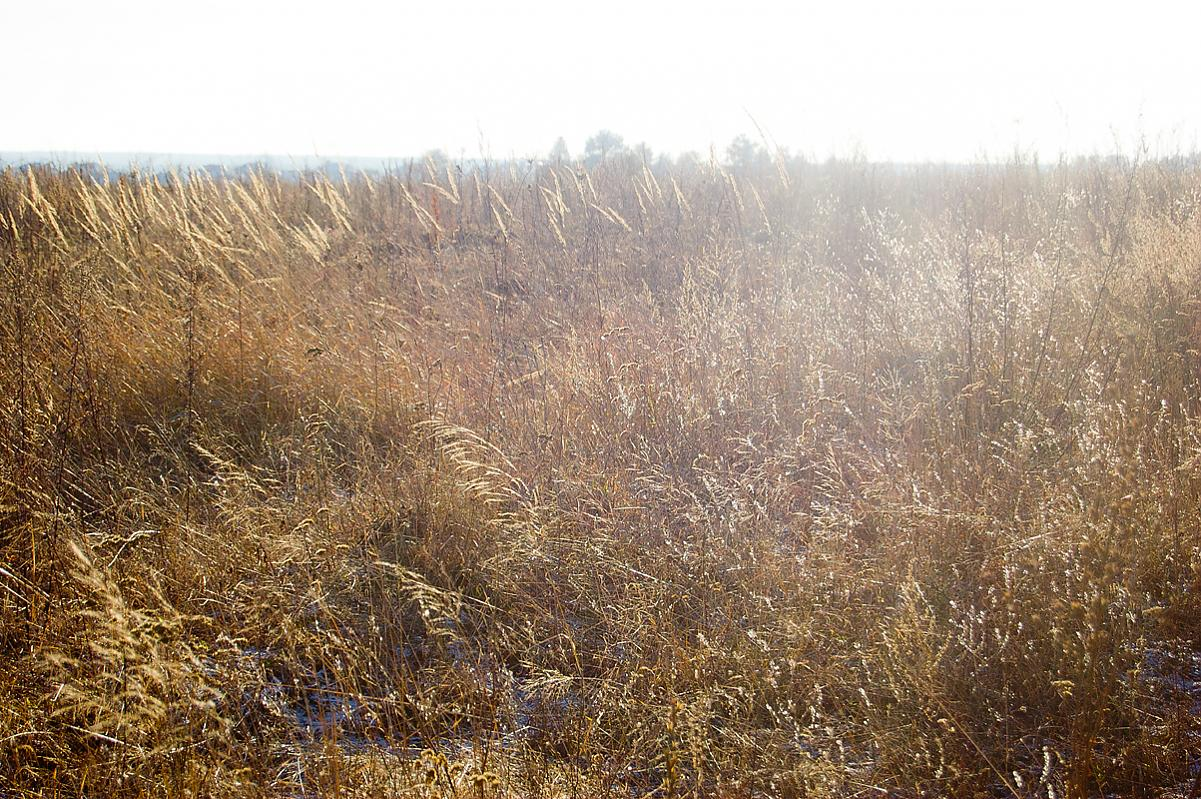
\includegraphics[width=\linewidth]{fogs/fog17.jpg} 
    \caption{}
    \label{fig:r17}
\end{figure}

\begin{figure}[H]
    \centering
    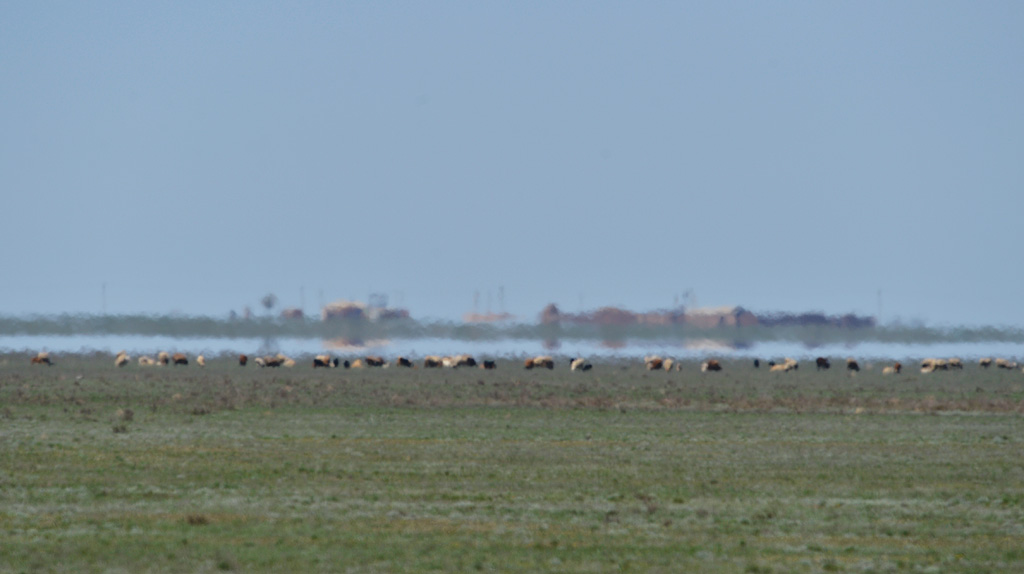
\includegraphics[width=\linewidth]{fogs/fog18.jpg} 
    \caption{}
    \label{fig:r18}
\end{figure}

\end{document}